% Memoria de la Parte 2 · Simulación de San Mamés (DMS, UJA 2026/27)
% Compilar con XeLaTeX (como la Parte 1):  latexmk -xelatex main.tex
% Fuentes de las cifras: Markdown de docs/memoria_parte2 (A1-A3, B1-B3, C1-C3),
% contrastados en INFORME_COHERENCIA.md con results/final y results/figures.
\documentclass[11pt,a4paper]{article}

% --- Idioma y fuentes (Inter, como la Parte 1) -------------------------------
\usepackage{fontspec}
\usepackage{unicode-math}
\setmainfont{Inter}[
  Extension=.otf, UprightFont=*-Regular, BoldFont=*-Bold,
  ItalicFont=*-Italic, BoldItalicFont=*-BoldItalic, Scale=0.92]
\newfontfamily\titlefont{Inter}[
  Extension=.otf, UprightFont=*-ExtraBold, BoldFont=*-Black, Ligatures=TeX]
\setmathfont{latinmodern-math.otf}
\usepackage[spanish,es-noshorthands,es-tabla]{babel}

% --- Página -------------------------------------------------------------------
\usepackage[a4paper,top=2.4cm,bottom=2.4cm,left=2.3cm,right=2.3cm,headheight=14pt]{geometry}
\usepackage{microtype}
\setlength{\parindent}{0pt}
\setlength{\parskip}{0.55em}
\linespread{1.08}

% --- Colores de la Parte 1 ----------------------------------------------------
\usepackage{xcolor}
\definecolor{marino}{rgb}{0.098,0.184,0.255}
\definecolor{azul}{rgb}{0.09,0.235,0.345}
\definecolor{turquesa}{rgb}{0.075,0.545,0.569}
\definecolor{gris}{rgb}{0.388,0.471,0.541}
\definecolor{grisclaro}{rgb}{0.796,0.843,0.875}

% --- Títulos de sección -------------------------------------------------------
\usepackage{titlesec}
\titleformat{\section}{\titlefont\Large\color{marino}}{\thesection.}{0.6em}{}
\titleformat{\subsection}{\bfseries\large\color{azul}}{\thesubsection.}{0.6em}{}
\titleformat{\subsubsection}{\bfseries\color{turquesa}}{}{0em}{}
\titlespacing*{\section}{0pt}{1.4em}{0.6em}
\titlespacing*{\subsection}{0pt}{1.1em}{0.4em}

% --- Cabecera y pie (como la Parte 1) -----------------------------------------
\usepackage{fancyhdr}
\pagestyle{fancy}
\fancyhf{}
\fancyhead[L]{\footnotesize\color{gris}DISEÑO DE MODELOS DE SIMULACIÓN}
\fancyhead[R]{\footnotesize\color{gris}PARTE 2 · SAN MAMÉS}
\fancyfoot[L]{\footnotesize\color{gris}UJA · CURSO 2026/2027}
\fancyfoot[R]{\footnotesize\color{gris}\thepage}
\renewcommand{\headrulewidth}{0.4pt}
\renewcommand{\headrule}{\color{grisclaro}\hrule height\headrulewidth}

% --- Tablas, figuras, listas, enlaces -----------------------------------------
\usepackage{booktabs,tabularx,array,longtable}
\usepackage{graphicx}
\graphicspath{{../../../results/figures/}}
\usepackage{float}
\usepackage[section]{placeins}
% Los flotantes no cruzan el inicio de un apartado.
\let\oldsubsection\subsection
\renewcommand{\subsection}{\FloatBarrier\oldsubsection}
\renewcommand{\topfraction}{0.9}
\renewcommand{\textfraction}{0.08}
\renewcommand{\floatpagefraction}{0.75}
% Las páginas solo de flotantes empiezan arriba, no centradas.
\makeatletter\setlength{\@fptop}{0pt}\setlength{\@fpsep}{1.2em}\makeatother
\usepackage[font=small,labelfont={bf,color=azul},labelsep=period]{caption}
\usepackage{subcaption}
\usepackage{enumitem}
\setlist{itemsep=0.2em,topsep=0.3em}
\usepackage{makecell}
\renewcommand{\cellalign}{tl}
\renewcommand{\theadfont}{\normalsize}
\usepackage{xurl}
\usepackage[hidelinks]{hyperref}
\hypersetup{
  pdftitle={Simulación del control de accesos, salida y gestión de incidencias en un estadio de fútbol. Parte 2},
  pdfauthor={Pablo Cuadros Rueda; Pablo Pérez Molina; José María Chamorro Bueno}}
\newcolumntype{Y}{>{\raggedright\arraybackslash}X}
\renewcommand{\arraystretch}{1.15}

% --- Macros -------------------------------------------------------------------
% Cifra que no se ha podido comprobar en el repositorio: se ve en rojo.
\newcommand{\pend}{\textcolor{red}{\textbf{PENDIENTE DE CONFIRMAR}}}
% Fecha de entrega: la pone Pablo Cuadros sustituyendo \pend por la fecha.
\newcommand{\fechaentrega}{\pend}

\begin{document}

% --- Portada (misma estructura que la Parte 1) --------------------------------
\begin{titlepage}
  \thispagestyle{empty}
  \centering
  {\color{gris}\small ESCUELA POLITÉCNICA SUPERIOR DE JAÉN\par}
  \vspace{0.4em}
  {\color{azul}\large\bfseries DISEÑO DE MODELOS DE SIMULACIÓN\par}
  \vspace{5.5cm}
  {\titlefont\color{marino}\huge Simulación del control de accesos, salida\\[0.2em]
   y gestión de incidencias en un estadio de\\[0.2em] fútbol\par}
  \vspace{1em}
  {\color{turquesa}\large Caso de referencia: Estadio de San Mamés Bilbao\par}
  \vspace{0.6em}
  {\color{gris}\large Parte 2 · Implementación, verificación y resultados\par}
  \vfill
  \begin{tabular}{@{}l@{\hspace{3em}}l@{}}
    {\color{gris}\small INTEGRANTES} & {\color{gris}\small HERRAMIENTA}\\[0.3em]
    Pablo Cuadros Rueda (pcr00036) & Python 3 + SimPy\\
    Pablo Pérez Molina (ppm00052) & \\[0.3em]
    José María Chamorro Bueno (jmcb0024) & {\color{gris}\small FECHA DE ENTREGA}\\
     & \fechaentrega\\
  \end{tabular}
\end{titlepage}

% Índice compacto: que quepa en una página, como en la Parte 1.
\begingroup\setlength{\parskip}{0pt}\linespread{0.95}\selectfont
\tableofcontents
\endgroup
\newpage

\section{Introducción}

En la Parte 1 se especificó un modelo de simulación de eventos discretos de la
entrada, la permanencia, la salida y las incidencias del público en el estadio
de San Mamés, con ocho preguntas (P1--P8) y un diseño experimental de escenarios
X0--X7 más una sensibilidad S1. Esta Parte 2 recoge el modelo implementado en
Python 3 con SimPy, su verificación y validación, y las respuestas a las ocho
preguntas.

La memoria se organiza así. La sección~\ref{sec:modelo} describe el modelo tal
como se ha implementado, y la sección~\ref{sec:desviaciones} reúne, con su
motivo, todo lo que difiere de la Parte 1. La sección~\ref{sec:verificacion}
explica cómo se calculan los indicadores, el método estadístico y la campaña de
réplicas, y las comprobaciones que dan confianza en el modelo. La
sección~\ref{sec:resultados} responde a P1--P8 en orden, la
sección~\ref{sec:sensibilidad} analiza la sensibilidad y la
sección~\ref{sec:conclusiones} cierra con las conclusiones y los límites.

\paragraph{Cómo leer las cifras.} Cada réplica es un partido completo. Salvo que
se indique otra cosa, las cifras son la media entre réplicas $\pm$ la
semianchura del intervalo de confianza (IC) del 95~\% (t de Student, una
observación por réplica), con el número de réplicas $n$. Las diferencias entre
escenarios están \emph{emparejadas}: se calculan réplica a réplica con la misma
semilla y $n$ es el número de parejas. Como no hay datos reales de colas ni de
salidas, los resultados se interpretan como comparaciones entre escenarios y no
como predicciones exactas de San Mamés, tal como advertía la Parte 1.

\section{Modelo implementado}\label{sec:modelo}

\subsection{Organización general}

El modelo se ha implementado en Python 3 con la librería SimPy, como preveía la
Parte 1. Es una simulación terminante: cada réplica es un partido completo, que
empieza con el estadio vacío al abrir las puertas en $t=-90$~min y termina
cuando todos los espectadores han salido o están a salvo. No hay periodo de
calentamiento, porque el estadio vacío es el estado inicial real y la entrada
forma parte de las preguntas. El reloj de SimPy trabaja en segundos con $t=0$ en
el inicio del partido; los resultados se expresan en minutos respecto a ese
instante. El final ordinario del partido es $t=+105$~min (90 de juego y 15 de
descanso).

Todos los parámetros están en un fichero de configuración. Cada experimento
declara solo lo que cambia respecto al escenario base, lo que hace explícito el
principio de la Parte 1 de cambiar un solo factor. La carga de la configuración
la valida y rechaza claves desconocidas, de modo que un error tipográfico no
produce en silencio un escenario distinto del previsto. Ningún parámetro del
modelo está escrito en el código.

Cada espectador es un único proceso que encadena entrada, ubicación,
permanencia y salida; la alarma de emergencia puede interrumpirlo para pasar a
la evacuación. Las averías de los tornos son procesos auxiliares que se repiten
indefinidamente y no determinan el fin de la réplica. Al terminar, la réplica
devuelve una fila por espectador con todos sus instantes, y los indicadores se
calculan a partir de esas filas (sección~\ref{sec:indicadores}).

\subsection{Generación de espectadores y llegadas}

Al empezar la réplica se generan los $N=48.775$ espectadores con todos sus
atributos:

\begin{itemize}
  \item \textbf{Hora de llegada.} Se sortea la franja de 15~min con las
    probabilidades del perfil (base o anticipado, tabla de la Parte 1) y un
    instante uniforme dentro de ella.
  \item \textbf{Macrozona, puerta y bloque.} Macrozona con un 25~\% de
    probabilidad cada una y, dentro de ella, puerta (1--6) y bloque (1--10)
    uniformes. Los bloques 1--5 forman la grada inferior y los 6--10 la
    superior.
  \item \textbf{Grupo.} Estándar (88~\%), mayores (10~\%) o personas con
    movilidad reducida, PMR (2~\%), con un factor de velocidad de 1, 0,8 y 0,5.
  \item \textbf{Velocidad, distancia y servicio.} Velocidad Normal(1,45;
    0,23)~m/s truncada en [0,6;~2,2] y multiplicada por el factor del grupo;
    distancia de la puerta al asiento Uniforme(60,~180)~m, que se usa también
    para salir; tiempo de servicio en el torno Triangular(2,~4,~6)~s.
\end{itemize}

Los espectadores se ordenan por hora de llegada. Cada atributo sale de su
propia fuente de números aleatorios (apartado~\ref{sec:nac}).

\subsection{Entrada: colas, tornos y prioridad}

Cada puerta es un recurso con tantas plazas como tornos (3 en el escenario
base) y una cola con prioridades. El espectador espera hasta su hora de
llegada, elige puerta (apartado~\ref{sec:cierre}), espera un torno libre y lo
ocupa durante su tiempo de servicio y, si le toca, la relectura de la entrada.
La espera en cola es el inicio del control menos la llegada.

Con la disciplina FIFO todos piden con el mismo nivel. Con prioridad (X3),
mayores y PMR piden con un nivel más alto y adelantan a los demás en la cola de
su puerta. La prioridad no es expulsiva: nunca interrumpe un control ya
iniciado. Dentro de cada nivel se mantiene el orden de llegada. Las averías
tienen un nivel aún más alto.

\subsection{Cierre de puerta y redirección}\label{sec:cierre}

En el experimento X6 la puerta 1 de la macrozona A se cierra durante 10~min
(cierre de puerta, I4). Mientras está cerrada nadie entra por ella. La puerta
se elige una sola vez, al llegar, con el estado de ese instante:

\begin{itemize}
  \item si la puerta asignada está abierta, el espectador va a ella;
  \item si está cerrada y la redirección está activa, va a la puerta abierta de
    su macrozona con menos cola (se desempata por personas en servicio y, después,
    por número de puerta; es una regla determinista, sin azar);
  \item si está cerrada y no hay redirección, espera a que reabra y entra después
    por su puerta, en el mismo orden en que llegaron quienes esperaban.
\end{itemize}

Quien se redirige no recorre ninguna distancia adicional, porque el modelo no
representa el exterior del estadio. Quien ya estaba en la cola de la puerta
cuando se cierra sigue siendo atendido; es una hipótesis adoptada que se discute
en la sección~\ref{sec:desviaciones}.

\subsection{Incidencias en el torno}

\textbf{Fallo de lectura (I2).} Con probabilidad 3~\%, al terminar el servicio
la entrada se vuelve a leer durante Uniforme(5,~15)~s más, sin liberar el torno.
La relectura no interrumpe ni es interrumpida.

\textbf{Avería de torno (I3).} Cada torno alterna periodos de funcionamiento
Exponencial(media 240~min) y reparaciones Uniforme(3,~10)~min. El tiempo entre
fallos se mide en funcionamiento: el reloj se detiene durante la reparación, de
modo que 240~min es el tiempo medio de buen funcionamiento y un torno no puede
averiarse mientras está parado. Al vencer ese tiempo, la avería pide el torno con
la prioridad máxima y sin expulsión: el torno termina el servicio en curso y
después se para, como indicaba la Parte 1 («cuando el torno queda libre»). La
avería adelanta a toda la cola, incluidos los grupos priorizados.

\subsection{Ubicación en el asiento y conflictos}

Tras el torno, el espectador camina hasta el vomitorio de su bloque a su propia
velocidad. Cada bloque tiene un vomitorio de 8 plazas atendidas por orden de
llegada; el paso dura Triangular(5,~10,~20)~s y al salir del vomitorio se sienta.

\textbf{Conflicto por asiento (I1).} Al llegar a su asiento, el espectador lo
encuentra ocupado con probabilidad 0,5~\% en el escenario base y 1~\% en el
experimento de acomodadores (X5). Mientras dura el conflicto no suelta su plaza
del vomitorio: pide un acomodador de su macrozona (6 en el escenario base),
espera si están todos ocupados y el conflicto se resuelve en Triangular(1,~3,~10)~min
desde que llega el acomodador. Retener la plaza es lo que hace que un conflicto
retrase también al resto del bloque: con varios conflictos a la vez, el
vomitorio pierde plazas y quienes vienen detrás esperan más (pregunta P6).

\subsection{Salida ordinaria}

Al final del partido cada macrozona dispone de 6 salidas de 4~m. Con 66 personas
por metro y minuto, cada salida deja pasar 264 personas por minuto, una cada
0,227~s. Cada espectador vuelve a recorrer su distancia y, al llegar a la zona de
salidas, elige la de su macrozona con menos personas en ese momento. Se han
simulado dos políticas: salida simultánea en $t=+105$ y salida escalonada (X4),
en la que la grada superior sale 3~min después que la inferior.

\subsection{Evacuación de emergencia}

En X7 suena una alarma en $t=+40$~min. Se cierran los accesos, las salidas se
ensanchan un 30~\% (de 4 a 5,2~m, una persona cada 0,175~s) y cada espectador
actúa según dónde está:

\begin{itemize}
  \item quien aún no ha llegado ya no llega y no cuenta en la evacuación;
  \item quien está en la cola exterior o pasando el torno abandona y tampoco cuenta;
  \item quien ya ha pasado el torno, esté caminando, en el vomitorio, en un
    conflicto o sentado, evacúa: espera su tiempo de reacción,
    Triangular(30,~60,~120)~s, camina un 20~\% más rápido hasta la salida de su
    macrozona con menos cola y la atraviesa.
\end{itemize}

En la variante con bloqueo, una de las 6 salidas de la macrozona A queda
inutilizada y su público se reparte entre las otras 5.

\subsection{Números aleatorios comunes}\label{sec:nac}

La Parte 1 pedía usar las mismas semillas en todos los escenarios y un generador
independiente por fuente de azar. La implementación va un paso más allá, porque
las mismas semillas no bastan si los números se asignan en distinto orden:

\begin{itemize}
  \item \textbf{Un generador por fuente.} Cada una de las 13 fuentes de azar
    (llegadas, asignación, grupo, velocidad, distancia, servicio, relectura,
    vomitorio, conflicto, avería, elección de salida, reacción y desempate de
    puerta) tiene su propio generador, derivado de la semilla de la réplica y de
    la posición fija de la fuente. Consumir más o menos números de una fuente no
    altera las demás.
  \item \textbf{Todo sorteo por espectador se hace al empezar la réplica.} Si el
    servicio o la relectura se sortearan durante la simulación con un generador
    compartido, cada número caería en un espectador distinto según el orden en
    que el modelo lo atiende, y ese orden cambia entre escenarios (por ejemplo,
    con 2 o 4 tornos). Por eso el servicio, la relectura y su duración, el paso
    por el vomitorio, el conflicto y su resolución, el desempate entre salidas y
    el tiempo de reacción se sortean una vez por espectador y quedan asociados a
    él. Además, conflicto y relectura se deciden comparando un uniforme con la
    probabilidad: al pasar del 0,5~\% al 1~\% de conflictos se conservan los de
    la base y solo se añaden otros, y las tres variantes de X5 tienen
    exactamente los mismos conflictos.
  \item \textbf{Un generador por torno para las averías.} El calendario de averías
    de cada torno es el mismo con 2, 3 o 4 tornos por puerta y no depende de las
    demás macrozonas.
  \item \textbf{Semilla de cada réplica:} $20261105+r$ para la réplica $r$
    (numerada desde 0), igual en todos los escenarios.
\end{itemize}

Así, la diferencia entre dos escenarios con la misma semilla se debe solo a lo
que cambia entre ellos. El efecto se comprueba en el
apartado~\ref{sec:reproducibilidad}.

\section{Desviaciones respecto a la Parte 1}\label{sec:desviaciones}

Esta sección reúne todo lo que difiere de la Parte 1. Se distinguen tres tipos:
correcciones de errores del texto de la Parte 1, cambios de diseño decididos por
el grupo e hipótesis que la Parte 1 no precisaba. Ninguna cambia la lógica del
modelo salvo las indicadas como cambios de diseño.

\begin{table}[htbp]
\centering
\small
\caption{Correcciones y cambios de diseño respecto a la Parte 1.}
\label{tab:desviaciones}
\begin{tabularx}{\textwidth}{@{}p{3.3cm}p{2.4cm}p{2.4cm}Y@{}}
\toprule
Aspecto & Parte 1 & Parte 2 & Motivo \\
\midrule
\multicolumn{4}{@{}l}{\textit{Correcciones del texto de la Parte 1}}\\
Intensidad de tráfico ρ del perfil anticipado (X2) & 0,65 & 0,81 &
La franja más cargada del perfil anticipado es la de $-45$ a $-30$~min
(24,4~\%, 793~pers/min), no la de $-30$ a $-15$. Con ella, $\rho = 793/978 \approx 0{,}81$.
No cambian el modelo ni los parámetros; los datos lo confirman
(apartado~\ref{sec:rho}). \\
Caso de 2 tornos por puerta & «la cola crece sin parar» & crece durante la punta &
La cola crece sin cota solo mientras dura la punta con $\rho>1$ (de $-30$ a 0~min);
después se vacía y todos entran. \\
\midrule
\multicolumn{4}{@{}l}{\textit{Cambios de diseño decididos por el grupo}}\\
Instante del cierre de puerta (X6) & $t=+20$~min & $t=-30$~min &
P7 pregunta por un cierre «en hora punta», pero en $t=+20$ llega solo el 2~\%
del público. En un estudio previo con 5 réplicas y seis instantes, la diferencia
sin\,$-$\,con redirección en la espera media de los asignados a la puerta cerrada
era de 4~$\pm$~1~s a $+20$ y de 292~$\pm$~24~s a $-30$, la mayor de las
probadas. Se mantienen la puerta (A-1) y la duración (10~min). \\
Acomodadores en X5 & 3 y 6 & 3, 6 y 9 &
Con 3 la cola de conflictos se satura. Se conservan la probabilidad del 1~\% y la
resolución Triangular(1,~3,~10)~min, y se añade un nivel de 9 para estudiar la
acumulación en lugar de ajustar los parámetros. \\
Número de réplicas & unas 30 por escenario & 30 a 247 &
Con el criterio de la propia Parte 1 (IC del 95~\% con semianchura $\le$~5~\% de la
espera media), el piloto estimó tamaños muy distintos. Se usan al menos 30 y el
tamaño necesario de cada escenario, comprobando la precisión al terminar
(apartado~\ref{sec:campana}). \\
\bottomrule
\end{tabularx}
\end{table}

\subsection{Hipótesis adoptadas}

La Parte 1 no precisaba los aspectos de la tabla~\ref{tab:hipotesis}. En cada
uno se ha elegido la lectura más sencilla y fiel al enunciado.

\begin{table}[htbp]
\centering
\small
\caption{Hipótesis adoptadas donde la Parte 1 no era explícita.}
\label{tab:hipotesis}
\begin{tabularx}{\textwidth}{@{}p{4.2cm}Y@{}}
\toprule
Aspecto & Hipótesis adoptada \\
\midrule
Cola formada al cerrar una puerta & Ver el párrafo siguiente. \\
Reloj de las averías & El tiempo entre fallos cuenta solo en funcionamiento;
240~min es el tiempo medio de buen funcionamiento. \\
Recuento de averías & Se cuentan todas las averías registradas en la réplica,
también las posteriores a la entrada. No equivale al número de averías que
perjudicaron a alguien. \\
Relectura y prioridad & La relectura no libera el torno; la prioridad no expulsa un
control en curso. \\
Utilización de los tornos & Se mide con el número nominal de tornos, desde la
apertura hasta el último control. Las averías cuentan como tiempo disponible no
ocupado. \\
Distancia en la evacuación & Quien está caminando hacia su asiento al sonar la
alarma recorre la distancia completa hasta la salida: no se conoce su posición y
es el caso más desfavorable. \\
Cola exterior al sonar la alarma & Quien está fuera, en cola o pasando el torno,
abandona y no cuenta en la evacuación. \\
Salida bloqueada & Se bloquea la salida 1 de la macrozona A; las 6 son iguales,
así que la elección no cambia el resultado. \\
Elección de salida & Se elige al llegar a la zona de salidas, cuando se ven las
colas, y no al levantarse. \\
Conflicto en curso al sonar la alarma & Se da por terminado: el espectador deja el
asiento para evacuar. \\
\bottomrule
\end{tabularx}
\end{table}

\paragraph{Cola formada al cerrar una puerta.}
Hipótesis adoptada: el cierre solo afecta a quien \emph{llega} mientras la puerta
está cerrada; quien ya estaba en su cola o en un torno sigue siendo atendido. Es
la lectura literal de la Parte 1 («nadie entra por esa puerta», «las llegadas se
redirigen o esperan»), que no trata la cola existente. La alternativa, parar
también esa cola, daría un efecto mayor del cierre. Con el cierre en $t=-30$
apenas importa: en el estudio previo había 0 o 2 personas en cola al cerrar,
frente a unas 380 llegadas durante el cierre, así que la hipótesis no influye
en X6. Con cierres más tardíos ($-20$, $-10$) llegaba a haber unas 100 personas
en cola al cerrar; para esos instantes no se ha comprobado y cambiar la
hipótesis obligaría a repetir X6.

Esta hipótesis va unida a una limitación de la redirección: quien llega a la
puerta cerrada conoce al instante la cola de todas las demás, elige la menor y no
camina ninguna distancia extra. La redirección del modelo es, por tanto,
optimista respecto a una real (apartado~\ref{sec:p7}).

\section{Verificación, validación y diseño estadístico}\label{sec:verificacion}

La Parte 1 fijó cinco criterios de verificación y validación: conservación,
orden temporal, capacidad de los recursos, casos límite y ritmo de paso por
torno. Como no hay datos reales de colas ni de salidas, la validación consiste en
comprobar que el modelo reproduce la comprobación previa de capacidad de la
Parte 1 y las distribuciones que esta fija, y que se comporta como predice la
teoría de colas. Antes se explica cómo se obtienen los indicadores y con qué
método estadístico se analizan.

\subsection{Indicadores}\label{sec:indicadores}

Los indicadores se calculan primero dentro de cada partido y después se analizan
entre partidos. Así no se trata a los miles de espectadores de una réplica, que
comparten colas y recursos, como si fueran observaciones independientes.

\begin{table}[htbp]
\centering\small
\caption{Cálculo de los indicadores dentro de una réplica.}
\label{tab:indicadores}
\begin{tabularx}{\textwidth}{@{}p{3.6cm}Yp{2.1cm}@{}}
\toprule
Indicador & Cálculo dentro de una réplica & Unidad \\
\midrule
Espera media y percentil 95 & Inicio del control menos llegada a la cola; media y percentil 95 de las esperas & min \\
Espera menor de 10~min & Porcentaje de personas con espera estrictamente menor de 10~min & \% \\
Cola máxima en una puerta & Mayor número de personas esperando a la vez en una puerta realmente usada & personas \\
Utilización de los tornos & Tiempo de servicio acumulado entre (tornos nominales $\times$ tiempo desde la apertura hasta el último control) & \% \\
Tiempo de acceso & Asiento menos llegada a la cola & min \\
Entrada tardía & De quienes llegan antes de $t=0$, porcentaje que se sienta después de $t=0$ & \% \\
Retraso por conflicto al resto del bloque & Diferencia del tiempo vomitorio--asiento entre otros espectadores expuestos y no expuestos a un conflicto en su bloque; excluye a quien lo causa & s por persona \\
Vaciado ordinario & Última salida menos final del partido & min \\
Máximo en una salida & Mayor número de personas a la vez en una salida, incluida la que la cruza & personas \\
Evacuación & Último en zona segura menos alarma; porcentaje a salvo a los 8~min & min; \% \\
\bottomrule
\end{tabularx}
\end{table}

Tres aclaraciones evitan lecturas erróneas:

\begin{itemize}
  \item La \textbf{entrada tardía} incluye control, marcha, vomitorio y posibles
    conflictos. La Parte 1 la llamaba «entrada tardía por colas», pero su
    definición no permite atribuir el retraso solo a la cola del torno; aquí se
    llama simplemente entrada tardía.
  \item La \textbf{utilización} promedia unas dos horas, desde la apertura hasta
    el último control. En X0 es del 40,43~\%, mientras que la intensidad de
    tráfico en la media hora punta es $\rho=0{,}93$: son ventanas y magnitudes
    distintas, y para la carga en la punta sirve $\rho$.
  \item El \textbf{percentil 95} publicado es la media entre réplicas de los
    percentiles de cada partido; la cola máxima es la media de los máximos por
    réplica. No se mezclan los espectadores de varias réplicas.
\end{itemize}

En P4 los mayores y las PMR se identifican con los mismos criterios en FIFO y
con prioridad, de modo que X0 y X3 comparan los mismos colectivos. En P7 se
distinguen la espera de todo el público y la del colectivo asignado a la puerta
A-1 que llega durante el cierre. En P8 el denominador del porcentaje a salvo es
la población que estaba dentro al sonar la alarma, aunque estuviera en tránsito;
quienes abandonan fuera o aún no han llegado no cuentan. Los indicadores que no
aplican a un escenario quedan sin valor y no cuentan en $n$.

\subsection{Método estadístico y campaña}\label{sec:campana}

\paragraph{Intervalos de confianza.} Para un indicador con valores
$Y_1,\dots,Y_n$ por réplica se calcula la media $\bar Y$ y el intervalo
t de Student del 95~\%:
\[
  \bar Y \pm h, \qquad h = t_{0{,}975;\,n-1}\,\frac{s}{\sqrt n}, \qquad
  s^2 = \frac{1}{n-1}\sum_{r=1}^n (Y_r-\bar Y)^2 .
\]
La semianchura $h$ describe la incertidumbre de la media entre réplicas, no la
dispersión entre espectadores ni un límite que todos los partidos respeten.

\paragraph{Diferencias emparejadas.} Para cada semilla común se calcula
$D_r = Y_{\text{alternativa},r} - Y_{\text{referencia},r}$ y se aplica la misma
fórmula a los $D_r$; $n$ es el número de parejas, que puede ser menor que el
tamaño de una de las muestras. Restar las medias de dos muestras completas no da
el mismo estimador. Las referencias son X0 para X1--X4 y S1, 6 acomodadores para
X5, sin redirección para X6 y todas las salidas para X7. Una diferencia negativa
reduce el indicador. Los IC son individuales para cada comparación; no son una
garantía simultánea para todos los indicadores.

\paragraph{Tamaño de muestra.} Se partió de 10 réplicas piloto por escenario y
se estimó el tamaño necesario para que la semianchura de la espera media no
superase el 5~\% de su valor:
$n = \lceil (t\,s/h_{\text{obj}})^2\rceil$ con $h_{\text{obj}} = 0{,}05\,|\bar Y|$,
con un mínimo de 30. Al terminar se recalculó el intervalo y se amplió la
muestra donde hacía falta. La precisión se fijó para la espera media de entrada,
no para cada indicador.

\begin{table}[htbp]
\centering\small
\caption{Réplicas definitivas por escenario y precisión alcanzada en la espera media.}
\label{tab:replicas}
\begin{tabular}{@{}lrr@{\hspace{2.5em}}lrr@{}}
\toprule
Escenario & $n$ & $h$ relativa (\%) & Escenario & $n$ & $h$ relativa (\%) \\
\midrule
X0 (base) & 180 & 4,34 & X6 (sin redirección) & 45 & 4,37 \\
X1 (2 tornos) & 30 & 1,93 & X6 (con redirección) & 199 & 3,71 \\
X1 (4 tornos) & 183 & 4,69 & X7 (todas las salidas) & 180 & 4,34 \\
X2 (llegada anticipada) & 138 & 4,97 & X7 (una salida bloqueada) & 180 & 4,34 \\
X3 (prioridad) & 181 & 4,32 & S1 (aforo $-$10~\%) & 247 & 4,19 \\
X4 (salida escalonada) & 180 & 4,34 & S1 (aforo $+$10~\%) & 73 & 4,50 \\
X5 (3 acomodadores) & 180 & 4,34 & S1 (velocidad $-$15~\%) & 180 & 4,34 \\
X5 (6 acomodadores) & 180 & 4,34 & S1 (velocidad $+$15~\%) & 180 & 4,34 \\
X5 (9 acomodadores) & 180 & 4,34 & S1 (servicio $-$25~\%) & 219 & 4,99 \\
 & & & S1 (servicio $+$25~\%) & 30 & 3,56 \\
\bottomrule
\end{tabular}
\end{table}

La campaña suma 2.965 réplicas en 19 escenarios: 13 configuraciones principales y
6 de sensibilidad. Todas cumplen el criterio, con una semianchura relativa máxima
del 4,9865~\%. Las 10 réplicas piloto de cada escenario forman parte del total,
sin contarse dos veces. Los escenarios que no cambian la entrada repiten la
espera de X0 semilla a semilla (apartado~\ref{sec:reproducibilidad}) y por eso
comparten su tamaño y precisión. El antiguo piloto de X6 con el cierre en
$t=+20$ es histórico y no se mezcla con la campaña.

\subsection{Conservación, orden temporal y capacidad}

\begin{itemize}
  \item \textbf{Conservación.} Las pruebas automáticas comprueban que cada
    espectador está en un único estado en cada transición, que es la igualdad de
    la Parte 1 persona a persona y no solo en la suma. En los datos definitivos,
    en las 2.605 réplicas sin alarma todos los espectadores generados entran, se
    sientan y salen, sin ninguno pendiente; en las 360 réplicas de X7 todos quedan
    a salvo (a $t=+40$ ya no hay cola exterior y nadie abandona).
  \item \textbf{Orden temporal.} Se comprueba llegada $\le$ inicio del control
    $\le$ fin del control $\le$ llegada al vomitorio $\le$ asiento $\le$ salida.
  \item \textbf{Capacidad.} Ningún torno atiende a más personas que su
    capacidad, también con averías; nunca hay más de 8 personas en un vomitorio,
    un conflicto retiene su plaza, cada macrozona usa solo sus acomodadores y cada
    salida deja pasar una persona cada 0,227~s.
\end{itemize}

Las tablas agregadas de la campaña no permiten reconstruir cada transición de las
2.965 réplicas; esa evidencia procede de la auditoría hecha al simular, de las
pruebas automáticas y de las reproducciones individuales.

\subsection{Capacidad de los tornos}

La Parte 1 estimó la capacidad real de un torno en 13,6~pers/min: servicio medio
de $4 + 0{,}03\times 10 = 4{,}3$~s con la relectura, y un 97,4~\% del tiempo
operativo por las averías ($240/(240+6{,}5)$). El cálculo analítico reproduce
esas cifras: servicio medio 4,30~s, disponibilidad 0,974, 13,59~pers/min por
torno y 978~pers/min con los 72 tornos. En los datos de X0 ($n=180$) se
comprueban los dos componentes por separado:

\begin{table}[htbp]
\centering\small
\caption{Componentes de la capacidad en X0 ($n=180$).}
\label{tab:componentes}
\begin{tabular}{@{}lrr@{}}
\toprule
Componente & Teórico & Modelo (IC 95~\%) \\
\midrule
Espectadores con relectura & 3,00~\% & 3,001 $\pm$ 0,011~\% \\
Averías por réplica (72 tornos, de la apertura al final) & 59,4 & 60,1 $\pm$ 1,0 \\
\bottomrule
\end{tabular}
\end{table}

Ambos valores teóricos quedan dentro del intervalo. El ritmo resultante se midió
en los periodos con cola sostenida, en los que los tornos no paran por falta de
público: en una réplica de X1 con 2 tornos, idéntica a la de la campaña, salen
13,54~pers/min por torno, un 0,4~\% por debajo de los 13,59 teóricos. Sin
incidencias, el ritmo medido es de 14,98~pers/min (teórico 15,00). Los
vomitorios admiten 411~pers/min por macrozona frente a los 245 que dejan pasar los
tornos, de modo que no son un cuello de botella en la entrada sin conflictos.

\subsection{Intensidad de tráfico y espera}\label{sec:rho}

La intensidad de tráfico es $\rho = \lambda_{\text{pico}}/\text{capacidad}$, con
$\lambda_{\text{pico}}$ la tasa de llegadas en la franja más cargada. Para
contrastarla con la espera observada se construyó un \emph{modelo fluido} de cada
puerta: llegadas y servicio como caudales continuos, con la capacidad media de
13,59~pers/min por torno. Ignora la variabilidad: con $\rho<1$ predice espera
nula y con $\rho>1$ una espera que crece a ritmo $\rho-1$ (minutos de espera por
minuto de reloj) mientras dura la sobrecarga y que después se reduce hasta
vaciarse. La simulación debe quedar algo por encima.

\begin{table}[htbp]
\centering\small
\caption{Intensidad de tráfico frente a la espera (min). Espera fluida: modelo
determinista; observada: media de las réplicas con IC del 95~\%.}
\label{tab:rho}
\begin{tabular}{@{}lrrrrr@{}}
\toprule
Escenario & $n$ & $\rho$ & Espera fluida & Espera observada & Percentil 95 observado \\
\midrule
X1 (4 tornos) & 183 & 0,70 & 0 & 0,016 $\pm$ 0,001 & 0,076 $\pm$ 0,002 \\
X2 (llegada anticipada) & 138 & 0,81 & 0 & 0,050 $\pm$ 0,003 & 0,209 $\pm$ 0,012 \\
S1 (aforo $-$10~\%) & 247 & 0,84 & 0 & 0,090 $\pm$ 0,004 & 0,489 $\pm$ 0,032 \\
X0 (base) & 180 & 0,93 & 0 & 0,192 $\pm$ 0,008 & 1,150 $\pm$ 0,068 \\
S1 (aforo $+$10~\%) & 73 & 1,02 & 0,205 & 0,486 $\pm$ 0,022 & 2,438 $\pm$ 0,130 \\
S1 (servicio $+$25~\%) & 30 & 1,15 & 1,304 & 1,402 $\pm$ 0,050 & 4,919 $\pm$ 0,211 \\
X1 (2 tornos) & 30 & 1,40 & 3,826 & 4,016 $\pm$ 0,078 & 11,764 $\pm$ 0,266 \\
\bottomrule
\end{tabular}
\end{table}

\begin{itemize}
  \item \textbf{La espera crece con $\rho$.} En los ocho escenarios sin cierre y
    con entrada distinta, el orden de las esperas medias es exactamente el de
    $\rho$.
  \item \textbf{Con $\rho$ muy por debajo de 1} (X1 con 4 tornos, X2) la espera
    media es de 1 a 3~s: lo observado es solo la variabilidad.
  \item \textbf{Con $\rho \approx 0{,}93$} (X0) la espera media es de 11,5~s y el
    percentil 95 de 1,15~min. Hay picos de cola por la variabilidad, pero no
    acumulación sostenida.
  \item \textbf{Con $\rho \approx 1$} (aforo $+$10~\%) el fluido predice
    0,21~min y se observan 0,49: en el entorno de $\rho=1$ domina la variabilidad
    y el fluido es solo una cota inferior.
  \item \textbf{Caso límite saturado} (X1 con 2 tornos, $\rho=1{,}40$). La espera
    crece sin cota durante la punta ($-30$ a 0~min) y se vacía después. El fluido
    predice una espera máxima de $(\rho-1)\times 30 \approx 11{,}9$~min, dentro del
    intervalo del percentil 95 observado (11,764~$\pm$~0,266~min). La espera media
    coincide con una desviación del 5~\% (3,826 fluido frente a
    4,016~$\pm$~0,078 observado), y con el servicio $+$25~\% la desviación es
    del 7~\%; en ambos casos lo observado queda por encima, como se espera.
    Que un modelo construido con 13,59~pers/min reproduzca la espera de los
    escenarios saturados confirma de forma independiente la capacidad efectiva.
  \item \textbf{$\rho$ de X2 = 0,81.} La espera observada en X2 (0,050~min) queda
    entre la de $\rho=0{,}70$ (0,016) y la de $\rho=0{,}84$ (0,090), coherente con
    0,81 y no con el 0,65 de la Parte 1.
  \item \textbf{Cierre de puerta en $t=-30$} (X6). Para quienes llegan a A-1
    durante el cierre, el fluido predice 9,66~min sin redirección y se observan
    9,626~$\pm$~0,120 ($n=45$), dentro del intervalo. Con redirección predice
    0,59~min y se observan 0,543~$\pm$~0,026 ($n=199$): coincide con una
    desviación del 8~\%, en este caso por debajo, porque ir a la puerta con menos
    cola reparte mejor que el reparto igual que supone el fluido.
\end{itemize}

\subsection{Distribuciones de entrada}

Se regeneraron, sin simular, los espectadores de las réplicas de X0 (180) y X2
(138) con sus semillas, y se contrastaron con las proporciones de la Parte 1
mediante $\chi^2$:

\begin{table}[htbp]
\centering\small
\caption{Contraste $\chi^2$ de los repartos de entrada con la Parte 1.}
\label{tab:repartos}
\begin{tabular}{@{}lrrrr@{}}
\toprule
Reparto & Réplicas & \makecell[r]{Desviación\\máxima} & \makecell[r]{$p$ ($\chi^2$\\agregado)} & \makecell[r]{Réplicas\\con $p<0{,}05$} \\
\midrule
Perfil por franjas, X0 & 180 & 0,010 p.\,p. & 0,62 & 3,3~\% \\
Perfil por franjas, X2 & 138 & 0,018 p.\,p. & 0,37 & 3,6~\% \\
Grupos 88/10/2~\%, X0 & 180 & 0,015 p.\,p. & 0,28 & 5,0~\% \\
Macrozonas 25~\%, los 19 escenarios & 2.965 & 0,006 p.\,p. & 0,21 & 5,5~\% \\
\bottomrule
\end{tabular}
\end{table}

Ningún reparto se rechaza y la fracción de réplicas rechazadas al 5~\% ronda el
5~\%, lo esperado si las proporciones son las de la Parte 1. Las réplicas
regeneradas dan exactamente los recuentos por macrozona de la campaña.

\subsection{Salida y evacuación frente a la Parte 1}

Para aislar el paso por las salidas, una prueba usa una macrozona ($N/4$, unas
12.194 personas) que llega junta a las salidas, con 1~m de recorrido y 1~s de
reacción:

\begin{table}[htbp]
\centering\small
\caption{Paso por las salidas de una macrozona frente a la Parte 1.}
\label{tab:salidas}
\begin{tabular}{@{}llrrr@{}}
\toprule
Caso & Salidas & Paso por persona & Parte 1 & Modelo \\
\midrule
Salida ordinaria & 6 de 4~m & 0,227~s & 7,7~min & 7,7~min \\
Evacuación & 6 de 5,2~m & 0,175~s & 5,9~min & 5,9~min \\
Evacuación con una salida bloqueada & 5 de 5,2~m & 0,175~s & 7,1~min & 7,1~min \\
\bottomrule
\end{tabular}
\end{table}

Estas cifras miden solo el paso por las salidas. Los tiempos del partido completo
(sección~\ref{sec:resultados}) son mayores porque incluyen la marcha, la reacción
y el reparto aleatorio del público; no se han ajustado parámetros para que ambos
coincidan.

\subsection{Casos límite}

\begin{table}[htbp]
\centering\small
\caption{Casos límite comprobados con pruebas automáticas o réplicas específicas.}
\label{tab:limites}
\begin{tabularx}{\textwidth}{@{}p{5cm}Y@{}}
\toprule
Caso & Resultado \\
\midrule
Muchos tornos, sin incidencias & Espera prácticamente nula (percentil 95 $<$ 0,01~min) y exactamente 0 con la misma demanda \\
2 tornos ($\rho=1{,}40$) & La espera crece en la punta con pendiente $\rho-1\approx 0{,}40$~min por minuto (tolerancia 15~\%) \\
4 tornos ($\rho=0{,}70$) & Sin tendencia en la punta y espera media $<$ 0,1~min \\
2, 3 y 4 tornos & El percentil 95 y la utilización decrecen con el número de tornos \\
Cierre en $-30$ sin redirección & Espera de los afectados próxima al fluido ($\approx$ 9,7~min) \\
Cierre en $-30$ con redirección & Espera $<$ 1,5~min y al menos 5 veces menor que sin ella \\
Acomodadores casi ilimitados (5 réplicas) & La duración media de un conflicto baja a 4,62~min, la media teórica de la resolución (4,67): la saturación con pocos acomodadores se debe a que faltan, no a un error del modelo \\
X7 con todas las salidas, réplicas que no vacían en 8~min & Solo llega tarde una persona, siempre PMR y sin cola en la salida; sin las PMR, el vaciado nunca pasa de 7,36~min \\
\bottomrule
\end{tabularx}
\end{table}

\subsection{Reproducibilidad y números aleatorios comunes}\label{sec:reproducibilidad}

\begin{itemize}
  \item \textbf{Misma semilla, mismos resultados.} Se repitió una réplica de cada
    uno de los 19 escenarios con su semilla original: los 21 indicadores y los
    datos de auditoría coinciden en todos los casos. Repetir una réplica comprueba
    la reproducibilidad, pero no añade réplicas a la campaña.
  \item \textbf{Números comunes.} En los escenarios que no modifican la entrada
    (X4, X5 con 3, 6 y 9 acomodadores, las dos variantes de X7 y S1 de
    velocidad), los indicadores de entrada (espera media, percentil 95, cola
    máxima, relecturas) son idénticos a los de X0 en las 180 semillas comunes. El
    número de relecturas coincide también en X1, X2, X3 y X6.
  \item \textbf{Efecto sobre la precisión.} La correlación entre escenarios
    emparejados es siempre positiva, así que emparejar nunca empeora el intervalo
    de una diferencia. En X6 (con frente a sin redirección, correlación 0,94) la
    varianza de la diferencia baja al 7~\% de la que tendría con muestras
    independientes y el intervalo se estrecha 3,7 veces; entre X1 o X2 y X0 la
    ganancia es pequeña (de 1,07 a 1,20 veces), porque sus varianzas son muy
    distintas.
\end{itemize}

\subsection{Validación frente a la Parte 1}

\begin{table}[htbp]
\centering\small
\caption{Validación de coherencia con la comprobación previa de la Parte 1.}
\label{tab:validacion}
\begin{tabularx}{\textwidth}{@{}p{4.2cm}p{2.7cm}Yp{2.2cm}@{}}
\toprule
Magnitud & Parte 1 & Modelo & ¿Coincide? \\
\midrule
Servicio medio con relectura & 4,3~s & 4,30~s; relectura en el 3,001~$\pm$~0,011~\% & Sí \\
Torno operativo & 97~\% & 97,4~\%; 60,1~$\pm$~1,0 averías frente a 59,4 & Sí \\
Capacidad por torno & 13,6~pers/min & 13,59; 13,54 medido con cola & Sí \\
Capacidad total & 978~pers/min & 978 & Sí \\
$\rho$ con 2 / 3 / 4 tornos & 1,40 / 0,93 / 0,70 & 1,40 / 0,93 / 0,70 & Sí \\
$\rho$ de X2 & 0,65 & 0,81 & No: error de la Parte 1 \\
Vomitorios frente a tornos & 411 frente a 245~pers/min & 411 y 245 & Sí \\
Repartos de entrada & 25~\%; perfil; 88/10/2~\% & $\chi^2$, $p \ge 0{,}21$ & Sí \\
Paso por salidas & 7,7 / 5,9 / 7,1~min & 7,7 / 5,9 / 7,1~min & Sí \\
Instante del cierre & $t=+20$~min & $t=-30$~min & No: cambio decidido \\
Ritmo por torno según la fuente F2 & unos 4~s, 15~pers/min & 14,98~pers/min sin incidencias & Sí con la cifra que cita la Parte 1 \\
\bottomrule
\end{tabularx}
\end{table}

\paragraph{Límites de la validación.} La Parte 1 pedía comprobar que el ritmo por
torno coincide con la fuente F2. El contraste se ha hecho con la cifra que la
Parte 1 atribuye a F2 (unos 4~s por persona, 15~pers/min por torno); esa cifra no
se ha vuelto a comprobar en el artículo original, así que el contraste no es una
validación independiente de F2. En
general, la validación comprueba que el modelo hace lo que la Parte 1 especifica
y lo que predice la teoría de colas; no demuestra que reproduzca las colas reales
de San Mamés. El perfil de llegadas y los parámetros de las incidencias son
hipótesis: la verificación muestra que el modelo los aplica bien, no que sean
ciertos.

\section{Resultados: respuestas a P1--P8}\label{sec:resultados}

Cada pregunta se responde con una frase, las cifras con su IC y $n$, la figura
que la ilustra, la distinción entre lo que es un resultado del modelo y lo que
depende de supuestos, y sus limitaciones. Las figuras muestran medias entre
réplicas con barras de IC del 95~\%; los números de las figuras usan punto
decimal.

% ---------------------------------------------------------------------------
\subsection{P1 · Operativa actual y cuello de botella}

\textbf{Respuesta.} Con la operativa actual (X0: 3 tornos por puerta, FIFO,
perfil base y conflictos, relecturas y averías activas) las esperas en los
tornos son cortas y nadie espera 10~minutos, pero los tornos trabajan cerca de
su límite en la media hora punta y son el cuello de botella de la entrada.

\begin{table}[htbp]
\centering\small
\caption{Operativa actual (X0, $n=180$).}
\label{tab:p1}
\begin{tabular}{@{}lr@{}}
\toprule
Indicador & Valor \\
\midrule
Espera media en cola & 0,192 $\pm$ 0,008~min (unos 11,5~s) \\
Percentil 95 de la espera & 1,150 $\pm$ 0,068~min \\
Público que espera menos de 10~min & 100,0~\% en las 180 réplicas \\
Máximo de personas en la cola de una puerta & 135 $\pm$ 6 \\
Utilización de los tornos & 40,43 $\pm$ 0,01~\% \\
Tiempo de acceso (llegada a la cola $\to$ asiento) & 1,972 $\pm$ 0,008~min \\
Entrada tardía & 4,578 $\pm$ 0,052~\% \\
\bottomrule
\end{tabular}
\end{table}

\begin{figure}[htbp]
\centering
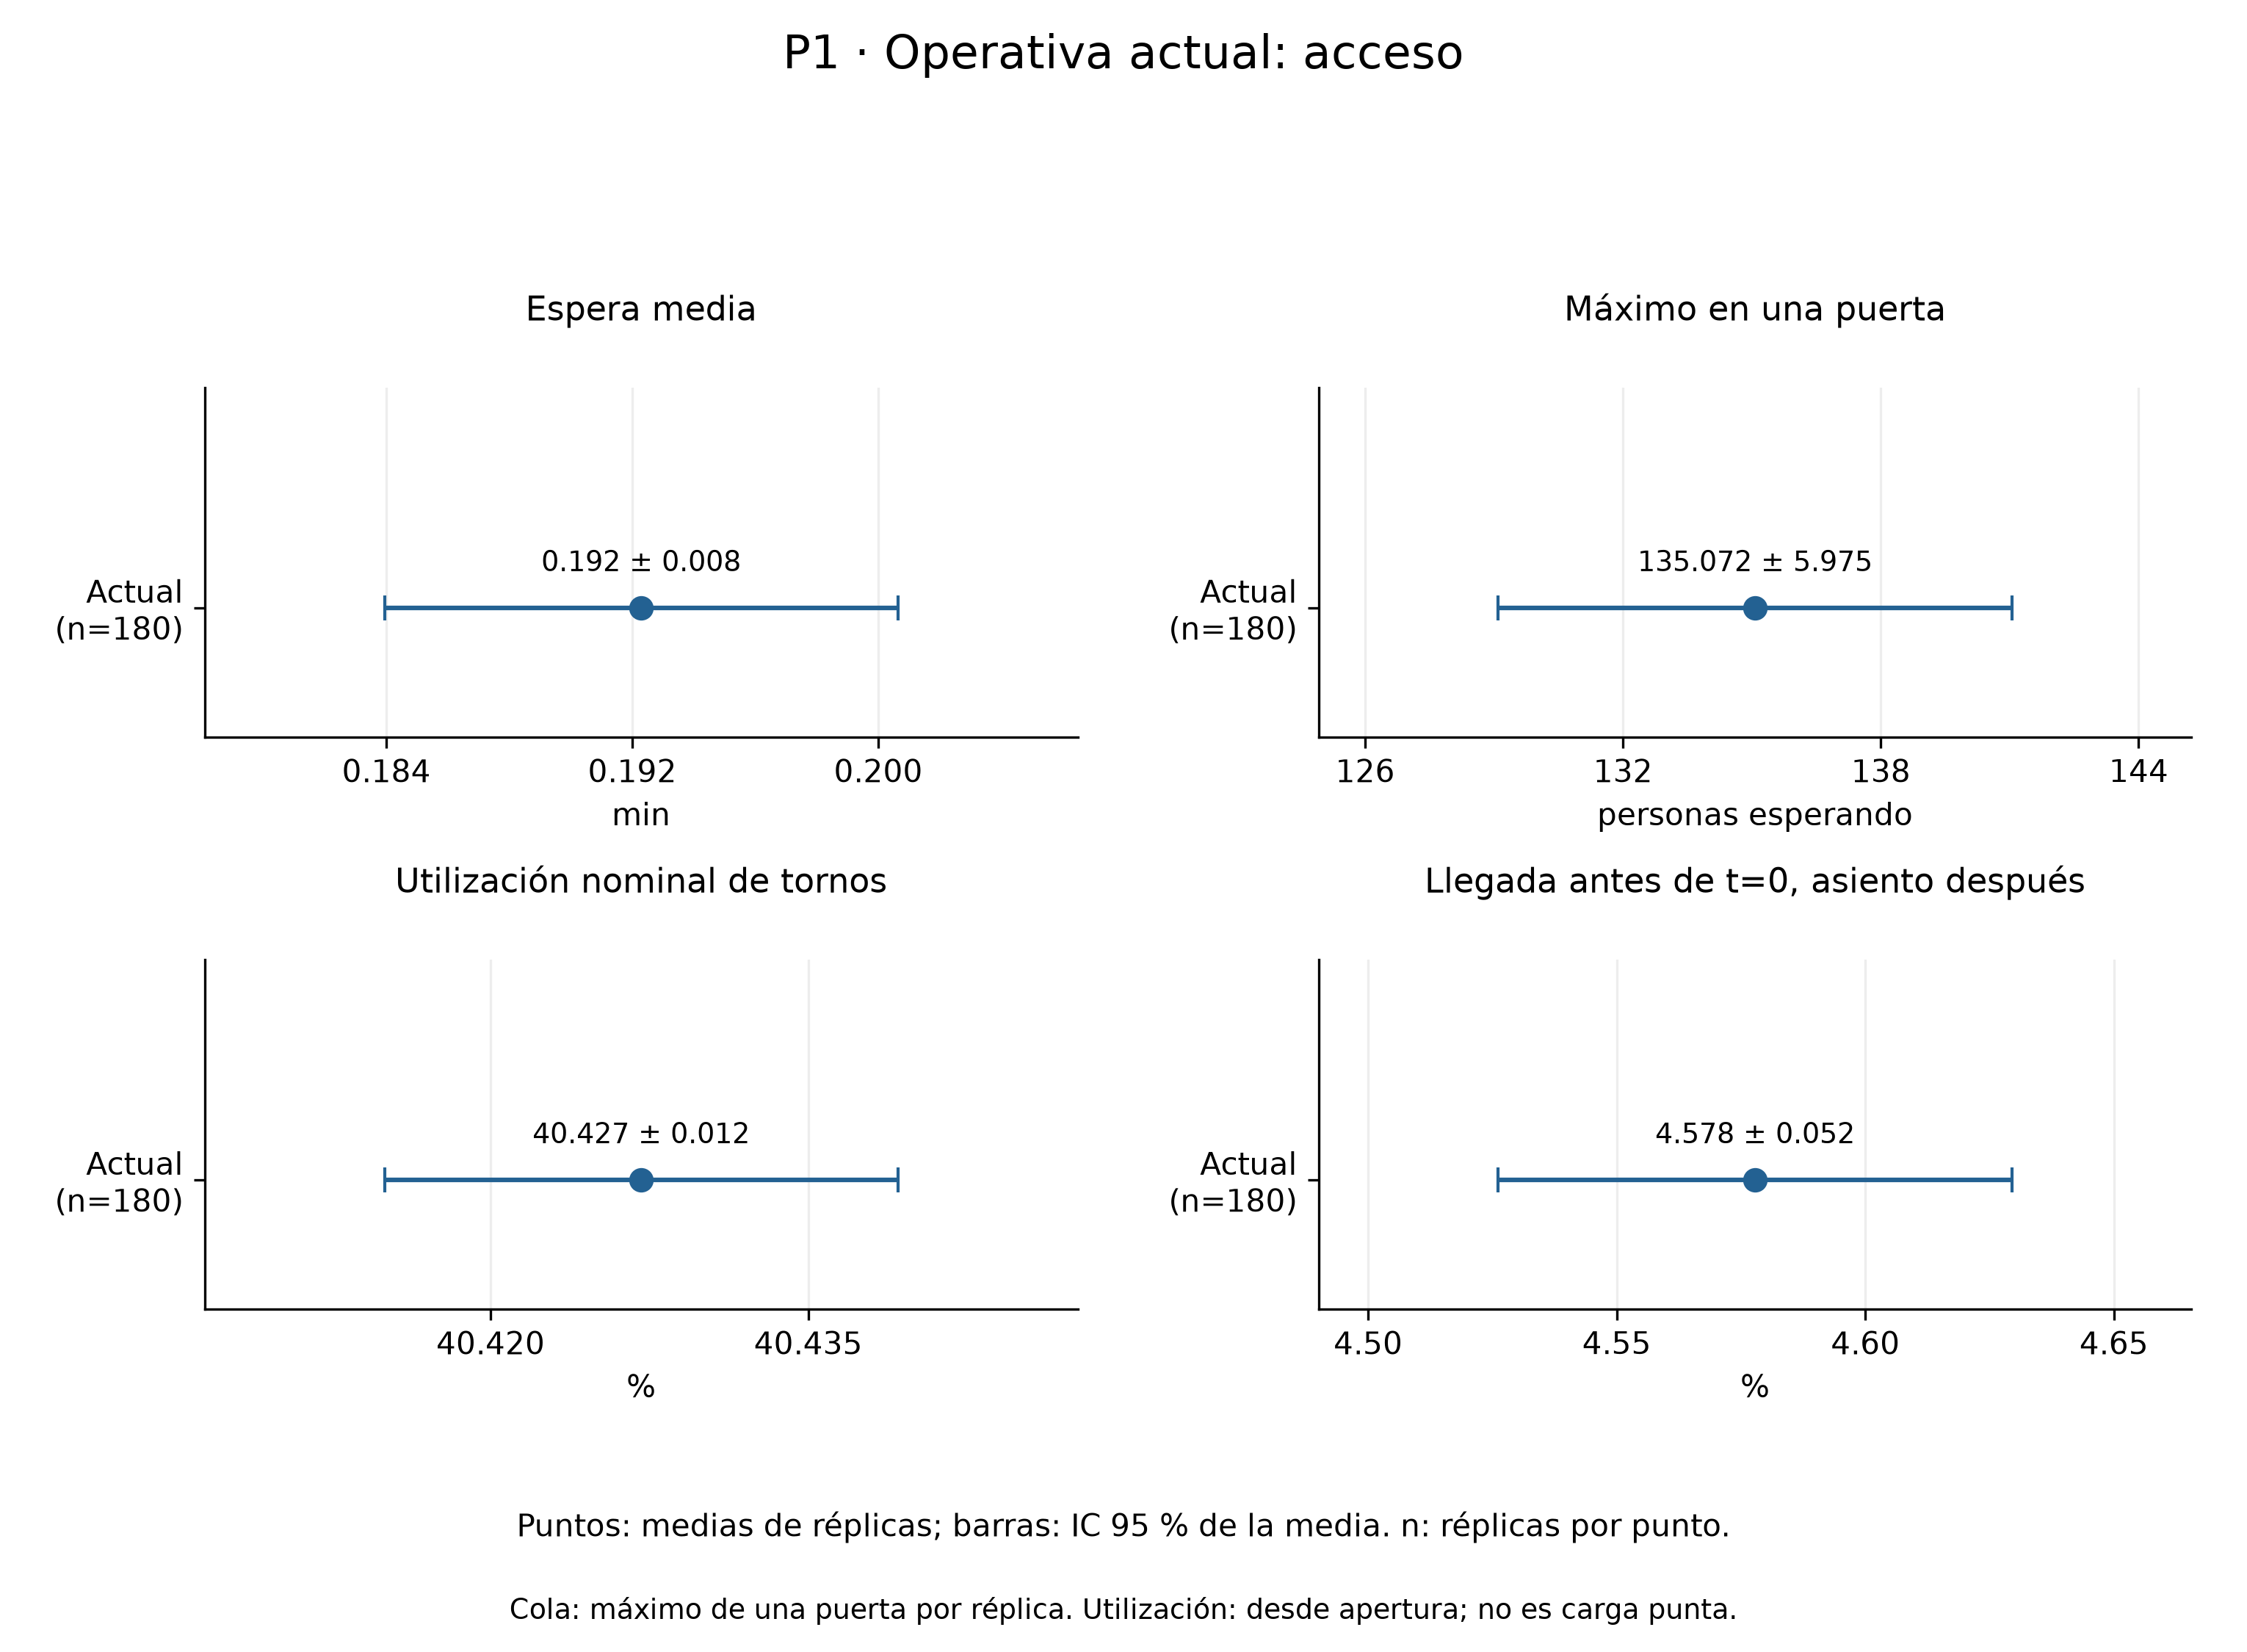
\includegraphics[width=\textwidth]{P1.png}
\caption{P1. Operativa actual (X0, $n=180$): espera media, máximo de personas
esperando en una puerta, utilización de los tornos y entrada tardía. Medias entre
réplicas con IC del 95~\%.}
\label{fig:p1}
\end{figure}

\textbf{Cuello de botella.} En la punta ($-30$ a 0~min) llegan 910~pers/min y los
72 tornos atienden 978: $\rho=0{,}93$. Los vomitorios admiten 411~pers/min por
macrozona frente a los 245 que dejan pasar los tornos, así que sin conflictos no
limitan la entrada. Con $\rho$ tan cerca de 1, pequeños cambios en la carga
tienen mucho efecto: con un 25~\% más de tiempo de servicio ($\rho=1{,}15$) la
espera media sube 1,217~$\pm$~0,034~min (30 parejas;
sección~\ref{sec:sensibilidad}).

\textbf{La entrada tardía no se debe sobre todo a la cola.} Con 4 tornos, donde la
espera es casi nula (0,016~$\pm$~0,001~min), sigue siendo del
3,754~$\pm$~0,016~\% ($n=183$); la diferencia emparejada con X0 es de
$-0{,}824 \pm 0{,}048$ puntos (180 parejas). Tampoco se debe a los conflictos: repitiendo X0 sin conflictos con las mismas
180 semillas, la entrada tardía baja del 4,578~\% al 4,488~\%, una diferencia
emparejada de 0,090~$\pm$~0,006 puntos, y el tiempo de acceso de 1,972 a
1,941~min, 0,032~$\pm$~0,001~min ($n=180$). Los conflictos explican menos del
2~\% de la entrada tardía. La mayor parte se explica, por tanto, por quienes
llegan en los últimos minutos y por el recorrido hasta el asiento.

\textbf{Resultado y supuestos.} Que los tornos sean el recurso más cargado y que la
espera sea corta con $\rho=0{,}93$ se sigue de los parámetros. Las cifras
absolutas dependen del número de tornos por puerta (3, una hipótesis de la Parte 1
porque el dato real no es público), del perfil de llegadas y del tiempo de
servicio, al que la espera es muy sensible.

\textbf{Limitaciones.} La utilización no describe la carga en la punta
(sección~\ref{sec:indicadores}) y los resultados agregados no permiten
reconstruir la cola a lo largo del reloj.

% ---------------------------------------------------------------------------
\subsection{P2 · Tornos por puerta}

\textbf{Respuesta.} Tres tornos por puerta, el valor actual, es el menor número
ensayado que cumple el objetivo de que el 95~\% del público espere menos de
10~minutos: con 3 y con 4 todo el público espera menos de 10~minutos en todas las
réplicas; con 2 no se alcanza el 95~\% en ninguna.

\begin{table}[htbp]
\centering\small
\caption{Tornos por puerta (X1 frente a X0).}
\label{tab:p2}
\begin{tabular}{@{}lrrrrrr@{}}
\toprule
Tornos & $n$ & $\rho$ & Espera $<$ 10~min & Espera media (min) & Percentil 95 (min) & Entrada tardía \\
\midrule
2 & 30 & 1,40 & 88,96 $\pm$ 0,74~\% & 4,016 $\pm$ 0,078 & 11,764 $\pm$ 0,266 & 20,30 $\pm$ 0,20~\% \\
3 & 180 & 0,93 & 100,0~\% & 0,192 $\pm$ 0,008 & 1,150 $\pm$ 0,068 & 4,58 $\pm$ 0,05~\% \\
4 & 183 & 0,70 & 100,0~\% & 0,016 $\pm$ 0,001 & 0,076 $\pm$ 0,002 & 3,75 $\pm$ 0,02~\% \\
\bottomrule
\end{tabular}
\end{table}

\begin{figure}[htbp]
\centering
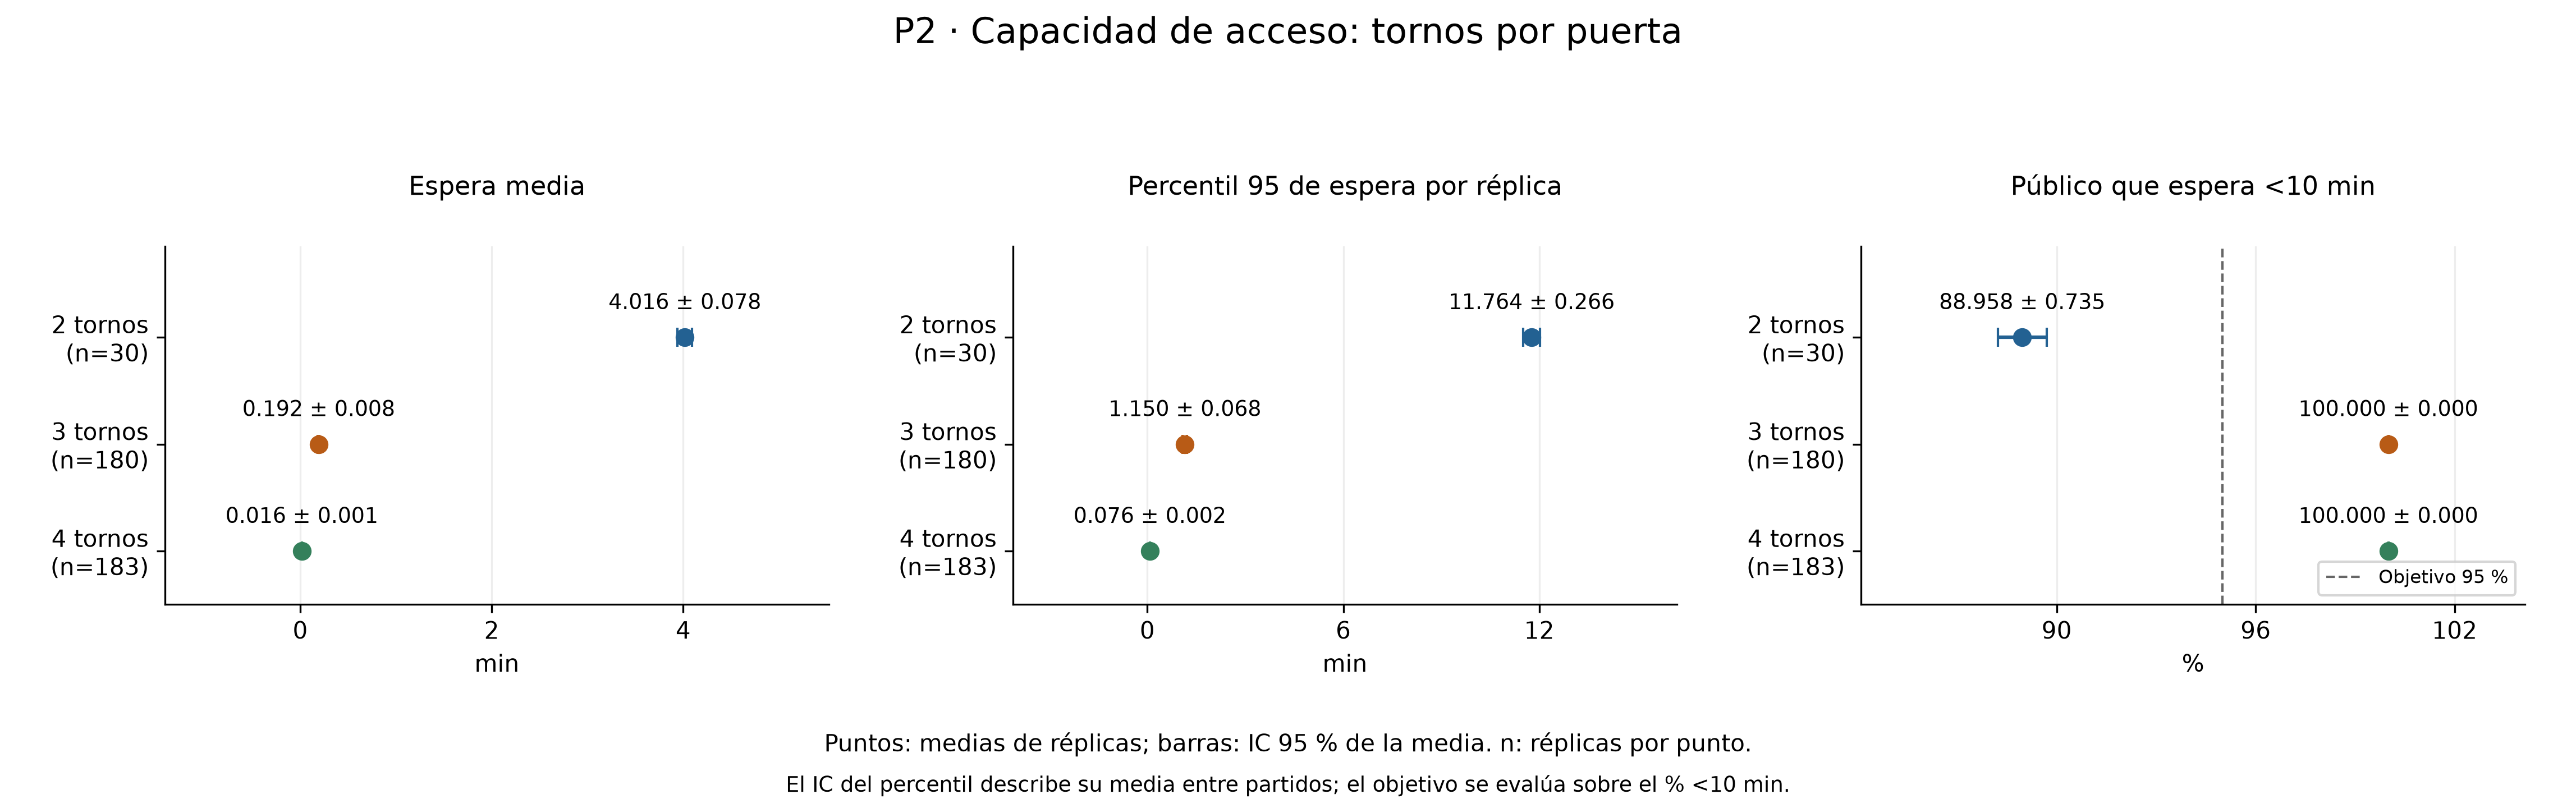
\includegraphics[width=\textwidth]{P2.png}
\caption{P2. Espera media, percentil 95 por réplica y público que espera menos
de 10~min con 2 ($n=30$), 3 ($n=180$) y 4 ($n=183$) tornos por puerta. Medias
con IC del 95~\%.}
\label{fig:p2}
\end{figure}

Con 2 tornos, el porcentaje que espera menos de 10~minutos va del 85,2~\% al
92,4~\% según la réplica: ninguna de las 30 llega al 95~\%. Frente a 3 tornos, la
espera media sube 3,832~$\pm$~0,067~min, el porcentaje bajo 10~minutos cae
11,04~$\pm$~0,74 puntos y la entrada tardía sube 15,79~$\pm$~0,19 puntos (30
parejas). La capacidad es menor que la demanda en la punta ($\rho=1{,}40$) y la
espera crece mientras dura, hasta unos 12~min; después la cola se vacía. Pasar de
3 a 4 tornos reduce la espera media en 0,176~$\pm$~0,008~min (unos 11~s) y la
entrada tardía en 0,82~$\pm$~0,05 puntos (180 parejas), pero no cambia el
cumplimiento del objetivo, que ya era del 100~\%.

\textbf{Robustez.} Con 3 tornos el objetivo se mantiene en las variantes de
sensibilidad: con un 10~\% más de público, 100,0~\% ($n=73$); con un 25~\% más
de tiempo de servicio ($\rho=1{,}15$), 99,931~$\pm$~0,045~\% ($n=30$), aunque el
percentil 95 sube a 4,919~$\pm$~0,211~min.

\textbf{Resultado y supuestos.} Que 2 tornos no basten y 3 sí es un resultado
robusto del modelo: se sigue de $\rho$ a un lado y otro de 1 y se mantiene en la
sensibilidad. El margen de 3 tornos depende del tiempo de servicio y del perfil
de llegadas, que son hipótesis.

\textbf{Limitaciones.} Solo se han ensayado 2, 3 y 4 tornos, iguales en todas las
puertas. El criterio se mide por partido simulado; que se cumpla en las 180
réplicas no garantiza que se cumpla en cualquier partido real.

% ---------------------------------------------------------------------------
\subsection{P3 · Llegada anticipada}

\textbf{Respuesta.} Si un 30~\% de quienes llegarían en los últimos 30~minutos
adelanta su llegada (X2), la espera media baja de unos 11,5 a unos 3~segundos y
la entrada tardía casi a la mitad, del 4,6~\% al 2,6~\%.

\begin{table}[htbp]
\centering\small
\caption{Llegada anticipada (X2, $n=138$) frente a X0 ($n=180$); diferencias con 138 parejas.}
\label{tab:p3}
\begin{tabular}{@{}lrrr@{}}
\toprule
Indicador & X0 & X2 & Diferencia X2 $-$ X0 \\
\midrule
Espera media (min) & 0,192 $\pm$ 0,008 & 0,050 $\pm$ 0,003 & $-$0,142 $\pm$ 0,009 \\
Percentil 95 de la espera (min) & 1,150 $\pm$ 0,068 & 0,209 $\pm$ 0,012 & $-$0,935 $\pm$ 0,078 \\
Máximo en la cola de una puerta & 135 $\pm$ 6 & 72 $\pm$ 5 & $-$63 $\pm$ 8 \\
Tiempo de acceso (min) & 1,972 $\pm$ 0,008 & 1,824 $\pm$ 0,003 & $-$0,149 $\pm$ 0,009 \\
Entrada tardía (\%) & 4,578 $\pm$ 0,052 & 2,604 $\pm$ 0,014 & $-$1,970 $\pm$ 0,054 p.\,p. \\
\bottomrule
\end{tabular}
\end{table}

\begin{figure}[htbp]
\centering
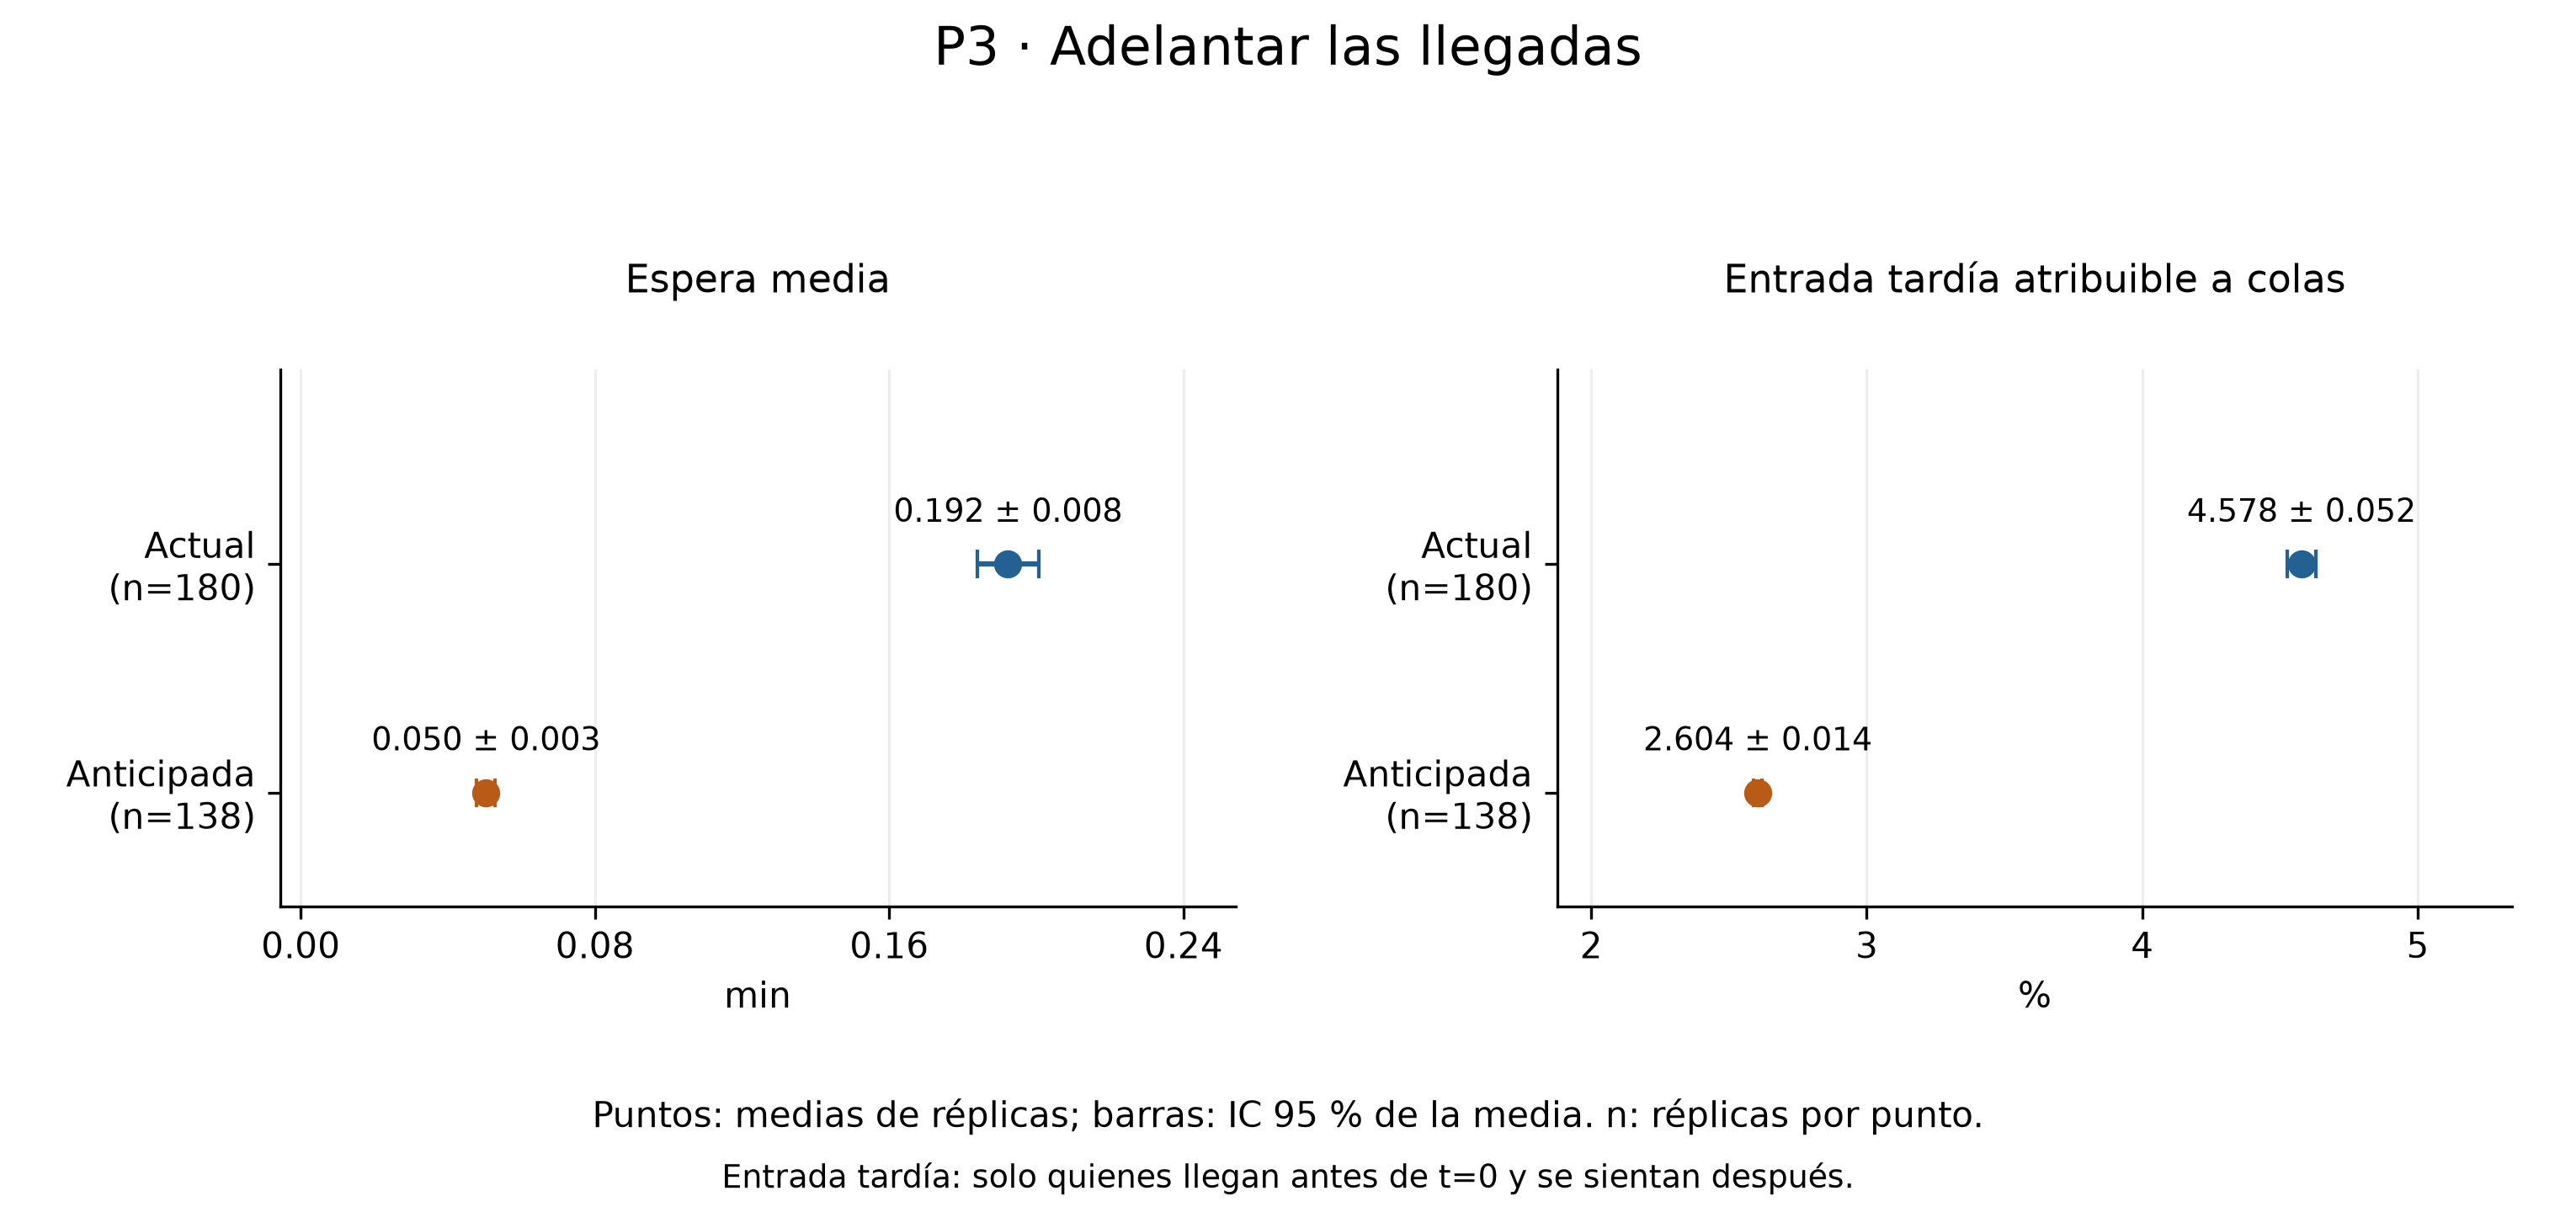
\includegraphics[width=0.92\textwidth]{P3.png}
\caption{P3. Espera media y entrada tardía con el perfil actual (X0, $n=180$) y
el anticipado (X2, $n=138$). Medias con IC del 95~\%. La entrada tardía incluye
el recorrido hasta el asiento.}
\label{fig:p3}
\end{figure}

La utilización no cambia (40,4~\%): el trabajo es el mismo, solo se reparte
mejor en el tiempo, y $\rho$ en la punta baja de 0,93 a 0,81. La entrada tardía
baja 1,97 puntos, más de lo que se gana al eliminar casi toda la cola con 4
tornos (0,82 puntos, P1): la mayor parte de la mejora viene de que menos gente
llega en los últimos minutos, no de la reducción de la cola. Esta lectura combina
dos contrastes distintos y es una inferencia, no una medida directa.

\textbf{Resultado y supuestos.} La dirección del efecto se sigue del modelo:
repartir las mismas llegadas en más tiempo reduce la carga en la punta. La
magnitud depende por completo del perfil anticipado, una hipótesis de la Parte 1
que no se ha calibrado con datos.

\textbf{Limitaciones.} El modelo no representa cómo se conseguiría que el público
llegue antes ni si un 30~\% es alcanzable. La mejora absoluta de la espera es
pequeña porque en X0 ya es corta; en un escenario más cargado, que no se ha
simulado, sería mayor.

% ---------------------------------------------------------------------------
\subsection{P4 · Prioridad para mayores y PMR}

\textbf{Respuesta.} Con prioridad no expulsiva en los tornos (X3), mayores y PMR
casi dejan de esperar (unos 11~s menos de media) y el resto espera unos 1,5~s
más; la espera media del conjunto no cambia.

\begin{table}[htbp]
\centering\small
\caption{Prioridad (mismos colectivos en X0, $n=180$, y X3, $n=181$; diferencias con 180 parejas).}
\label{tab:p4}
\begin{tabular}{@{}lrrr@{}}
\toprule
Colectivo & X0 (FIFO) & X3 (prioridad) & Diferencia X3 $-$ X0 \\
\midrule
Mayores y PMR, espera media (min) & 0,192 $\pm$ 0,008 & 0,0108 $\pm$ 0,0001 & $-$0,181 $\pm$ 0,008 \\
Resto, espera media (min) & 0,192 $\pm$ 0,008 & 0,217 $\pm$ 0,009 & $+$0,0248 $\pm$ 0,0011 \\
\bottomrule
\end{tabular}
\end{table}

\begin{figure}[htbp]
\centering
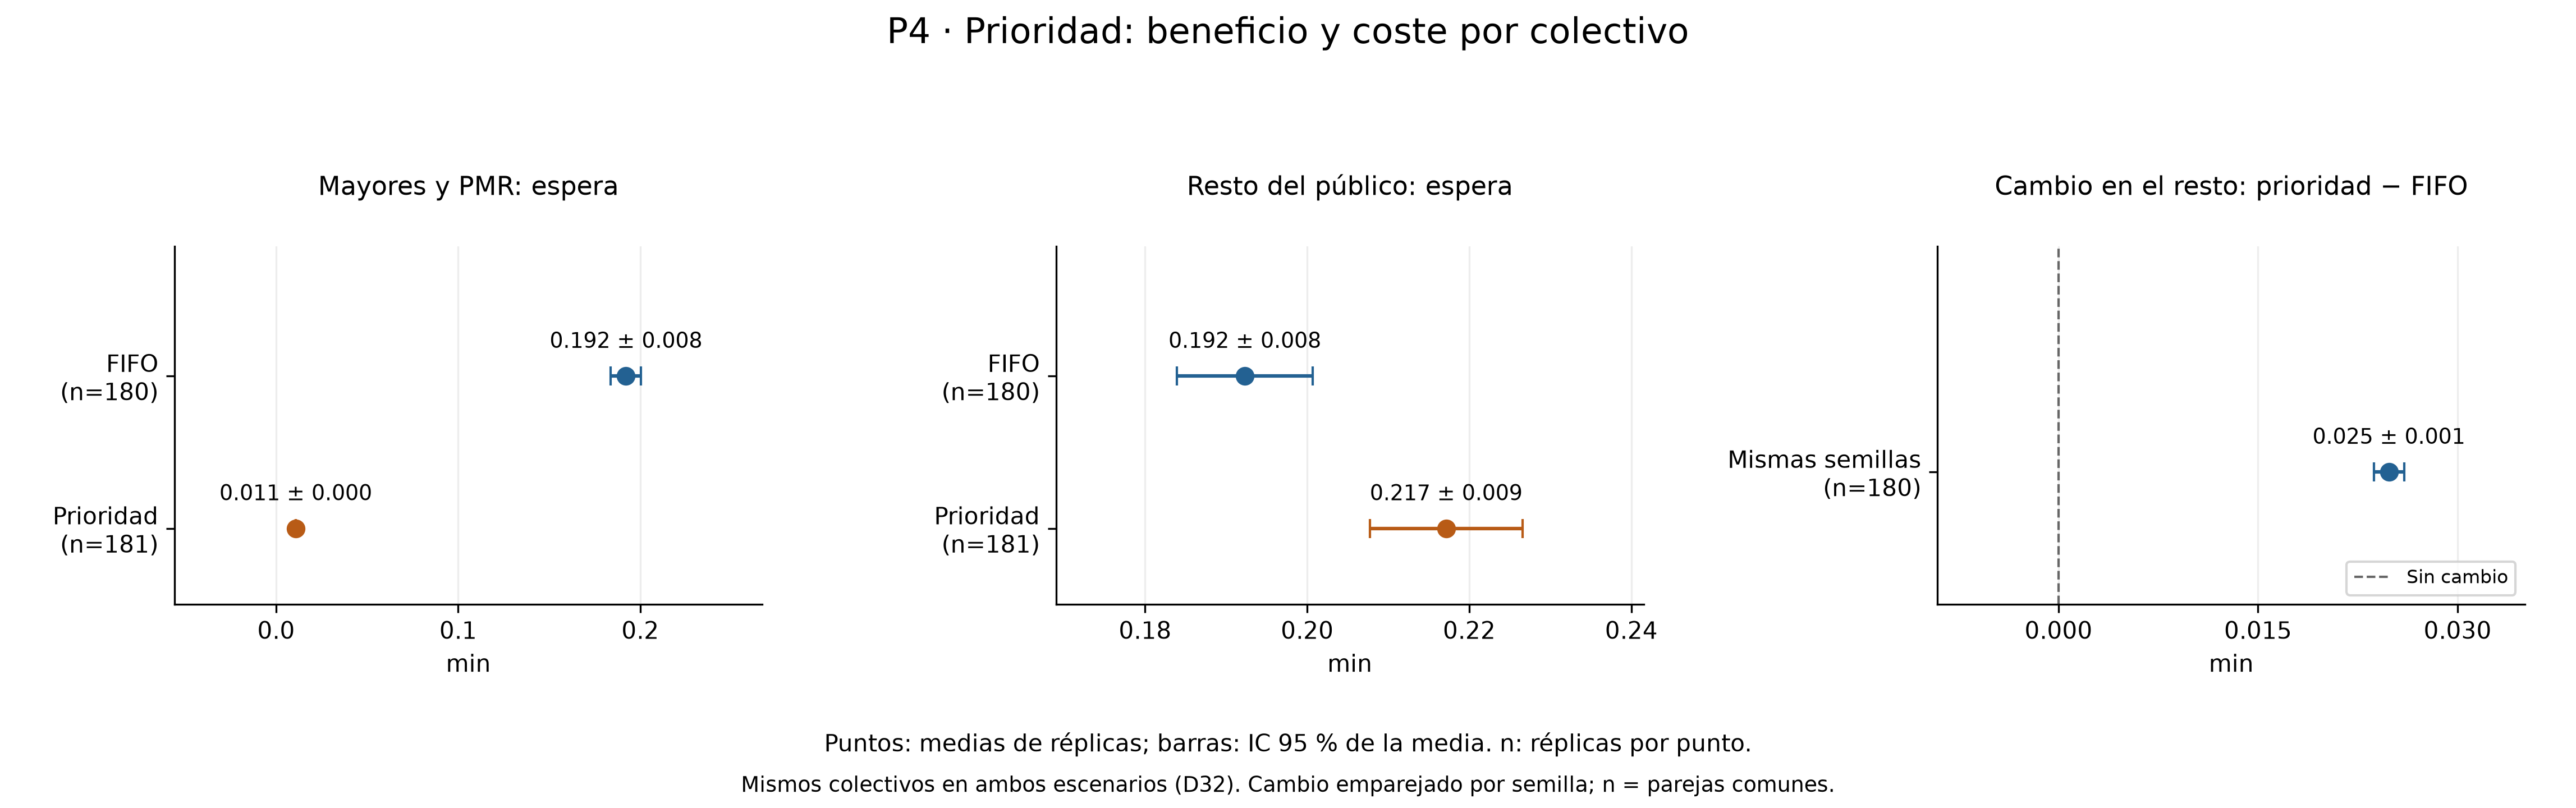
\includegraphics[width=\textwidth]{P4.png}
\caption{P4. Espera de mayores y PMR y del resto del público en FIFO (X0,
$n=180$) y con prioridad (X3, $n=181$), con los mismos colectivos; cambio
emparejado en el resto (180 parejas). Medias con IC del 95~\%.}
\label{fig:p4}
\end{figure}

En X3, la diferencia entre la espera de los priorizados y la del resto es de
$-0{,}206 \pm 0{,}009$~min ($n=181$). La espera media de todo el público no
cambia ($+0{,}00006 \pm 0{,}00007$~min; el intervalo incluye el cero), ni la
entrada tardía ($+0{,}0005 \pm 0{,}0028$ puntos): la prioridad reordena la cola
sin cambiar el trabajo de los tornos. La ganancia por persona priorizada es unas
siete veces la pérdida por persona del resto, porque el colectivo priorizado es
el 12~\% del público.

\textbf{Resultado y supuestos.} Que la espera total no cambie y que el coste se
reparta entre muchos es una propiedad de la prioridad no expulsiva con servicios
iguales. Las magnitudes absolutas son pequeñas porque la espera de X0 es corta;
con más carga, ganancia y pérdida serían mayores, pero no se ha simulado.

\textbf{Limitaciones.} La prioridad solo actúa en el torno, no en el vomitorio ni
en la salida. Se supone que el colectivo se identifica sin error ni coste al
llegar a la puerta. La movilidad reducida se representa solo con una velocidad
menor en el recorrido; el servicio en el torno es igual para todos.

% ---------------------------------------------------------------------------
\subsection{P5 · Salida escalonada}

\textbf{Respuesta.} Sí: con la salida escalonada (X4), el máximo de personas en
una salida baja casi a la mitad, a cambio de que el estadio tarde algo más de un
minuto más en vaciarse.

\begin{table}[htbp]
\centering\small
\caption{Salida simultánea (X0) frente a escalonada (X4), $n=180$ cada una; diferencias con 180 parejas.}
\label{tab:p5}
\begin{tabular}{@{}lrrr@{}}
\toprule
Indicador & Simultánea & Escalonada & Diferencia \\
\midrule
Máximo en una salida (personas) & 1.460,0 $\pm$ 1,3 & 746,1 $\pm$ 1,4 & $-$713,9 $\pm$ 0,6 \\
Vaciado desde el final del partido (min) & 8,367 $\pm$ 0,019 & 9,591 $\pm$ 0,108 & $+$1,224 $\pm$ 0,105 \\
\bottomrule
\end{tabular}
\end{table}

\begin{figure}[htbp]
\centering
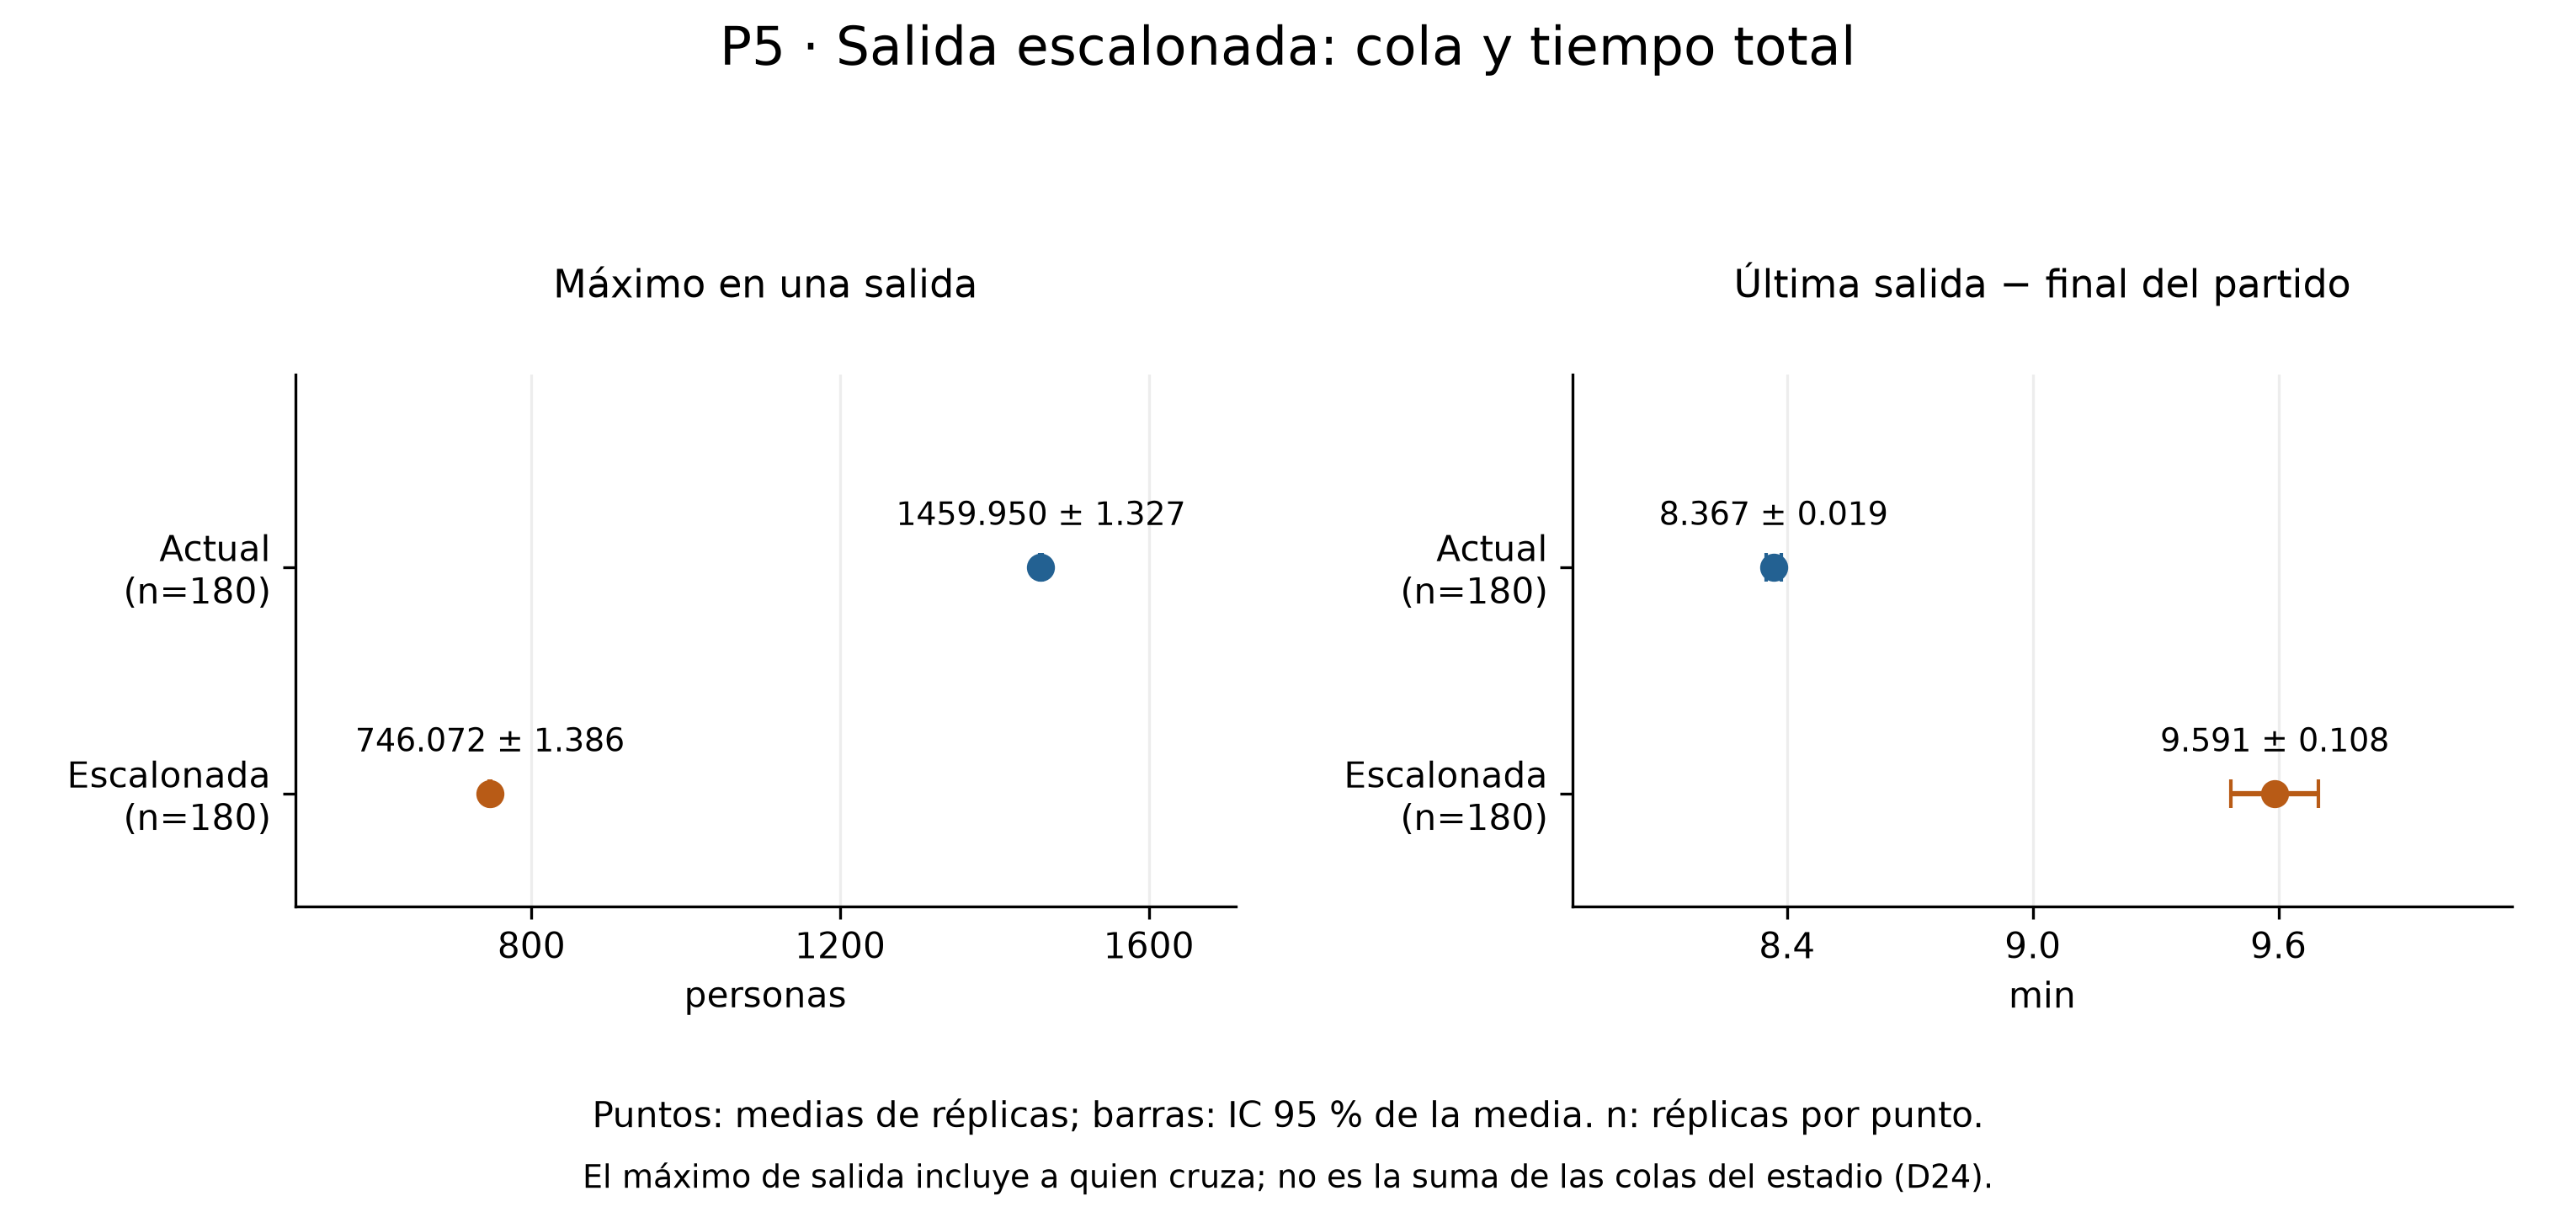
\includegraphics[width=0.92\textwidth]{P5.png}
\caption{P5. Máximo de personas en una salida y tiempo de vaciado con salida
simultánea (X0) y escalonada (X4), $n=180$ cada una. Medias con IC del 95~\%. El
máximo incluye a quien cruza la salida.}
\label{fig:p5}
\end{figure}

La salida escalonada reparte la carga en el tiempo: conviene si lo que preocupa
es la aglomeración en las salidas, no el tiempo total de vaciado. El máximo
incluye a quien está cruzando y no suma todas las colas del estadio. El vaciado
de X0 (8,367~min) supera los 7,7~min de la Parte 1 porque incluye la marcha hasta
la salida y la cola, que el cálculo de capacidad no considera.

% ---------------------------------------------------------------------------
\subsection{P6 · Conflictos por asiento y acomodadores}

\textbf{Respuesta.} Con conflictos al 1~\% el número de acomodadores es decisivo:
con 3 por macrozona el sistema se satura; con 6 todavía se forma cola, y de los
tres niveles probados solo con 9 la duración de un conflicto se acerca a la de la
propia resolución.

Con conflictos al 1~\% hay unos 490 conflictos por partido, unos 122 por
macrozona, concentrados en la hora punta, que exigen unos 569~min de trabajo de
acomodador por macrozona. Cada uno ocupa a un acomodador una media teórica de
4,67~min de resolución.

\begin{table}[htbp]
\centering\small
\caption{Acomodadores por macrozona con conflictos al 1~\% (X5, $n=180$ por nivel).}
\label{tab:p6}
\begin{tabular}{@{}lrrr@{}}
\toprule
Acomodadores & \makecell[r]{Duración media de\\un conflicto (min)} & \makecell[r]{Retraso al resto del\\bloque (s por persona)} & \makecell[r]{Entrada\\tardía (\%)} \\
\midrule
3 & 44,600 $\pm$ 0,477 & 291,7 $\pm$ 11,9 & 14,55 $\pm$ 0,28 \\
6 & 13,744 $\pm$ 0,206 & 36,8 $\pm$ 2,4 & 7,19 $\pm$ 0,14 \\
9 & 6,644 $\pm$ 0,092 & 6,7 $\pm$ 0,6 & 5,13 $\pm$ 0,07 \\
\bottomrule
\end{tabular}
\end{table}

\begin{figure}[htbp]
\centering
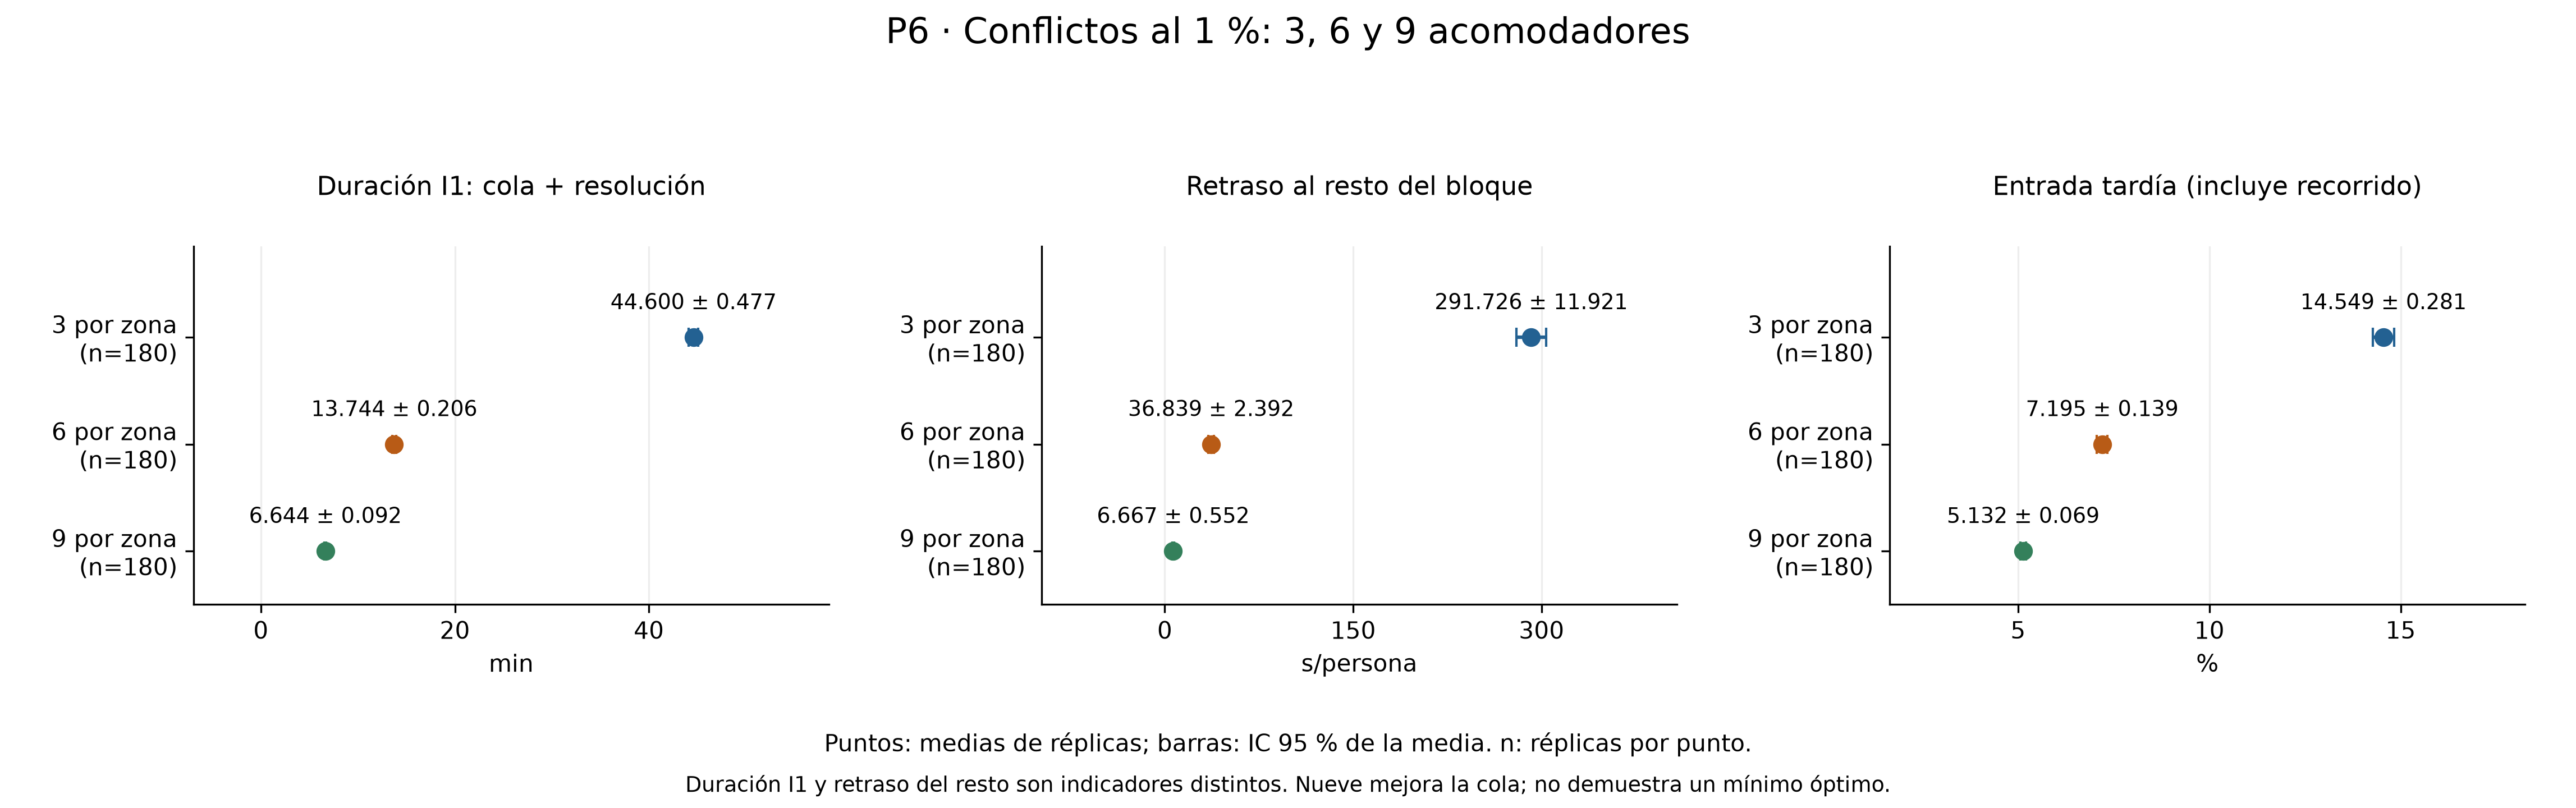
\includegraphics[width=\textwidth]{P6.png}
\caption{P6. Duración media de un conflicto (espera al acomodador más
resolución), retraso al resto del bloque y entrada tardía con 3, 6 y 9
acomodadores por macrozona ($n=180$ por nivel). Medias con IC del 95~\%.}
\label{fig:p6}
\end{figure}

Frente a 6 acomodadores, el retraso al resto del bloque aumenta
254,9~$\pm$~9,9~s por persona con 3 y baja 30,2~$\pm$~1,9 con 9 (180 parejas).
Con 3, los conflictos esperan mucho más de lo que tardan en resolverse y, en el
peor caso observado, el último espectador se sienta casi tres horas después del
inicio del partido. La duración media incluye la espera al acomodador, por eso
supera el rango de la resolución sin contradecir su distribución; con
acomodadores casi ilimitados vuelve a la media teórica (tabla~\ref{tab:limites}).

\textbf{Limitaciones.} El retraso al resto del bloque es una comparación entre
espectadores expuestos y no expuestos a un conflicto, no una medida causal del
mismo espectador con y sin conflicto. Nueve acomodadores mejoran mucho la
situación, pero no eliminan toda la cola ni demuestran que 9 sea el mínimo
necesario.

% ---------------------------------------------------------------------------
\subsection{P7 · Cierre de una puerta en hora punta}\label{sec:p7}

\textbf{Respuesta.} Sí, la redirección lo absorbe casi por completo. Si la puerta
A-1 se cierra 10~minutos al empezar la punta ($t=-30$), quienes llegan a ella
esperan de media unos 9,6~minutos sin redirección y medio minuto con ella.

El colectivo afectado son los asignados a A-1 que llegan durante el cierre:
383,3~$\pm$~5,6 de media sin redirección y 382,5~$\pm$~2,7 con ella; con
redirección se redirigen todos.

\begin{table}[htbp]
\centering\small
\caption{Cierre de A-1 en $[-30,-20)$~min: sin redirección ($n=45$) y con ella
($n=199$); diferencias con 45 parejas.}
\label{tab:p7}
\begin{tabular}{@{}lrrr@{}}
\toprule
Indicador & Sin redirección & Con redirección & Diferencia con $-$ sin \\
\midrule
Espera media del colectivo afectado (min) & 9,626 $\pm$ 0,120 & 0,543 $\pm$ 0,026 & --- \\
Espera media de todo el público (min) & 0,403 $\pm$ 0,018 & 0,243 $\pm$ 0,009 & $-$0,160 $\pm$ 0,007 \\
Máximo en la cola de una puerta & 395 $\pm$ 7 & 140 $\pm$ 6 & $-$258 $\pm$ 13 \\
Entrada tardía (\%) & 5,247 $\pm$ 0,108 & 4,645 $\pm$ 0,052 & $-$0,650 $\pm$ 0,029 p.\,p. \\
Público que espera $<$ 10~min (\%) & 99,717 $\pm$ 0,143 & 100,0 & $+$0,283 $\pm$ 0,143 \\
\bottomrule
\end{tabular}
\end{table}

\begin{figure}[htbp]
\centering
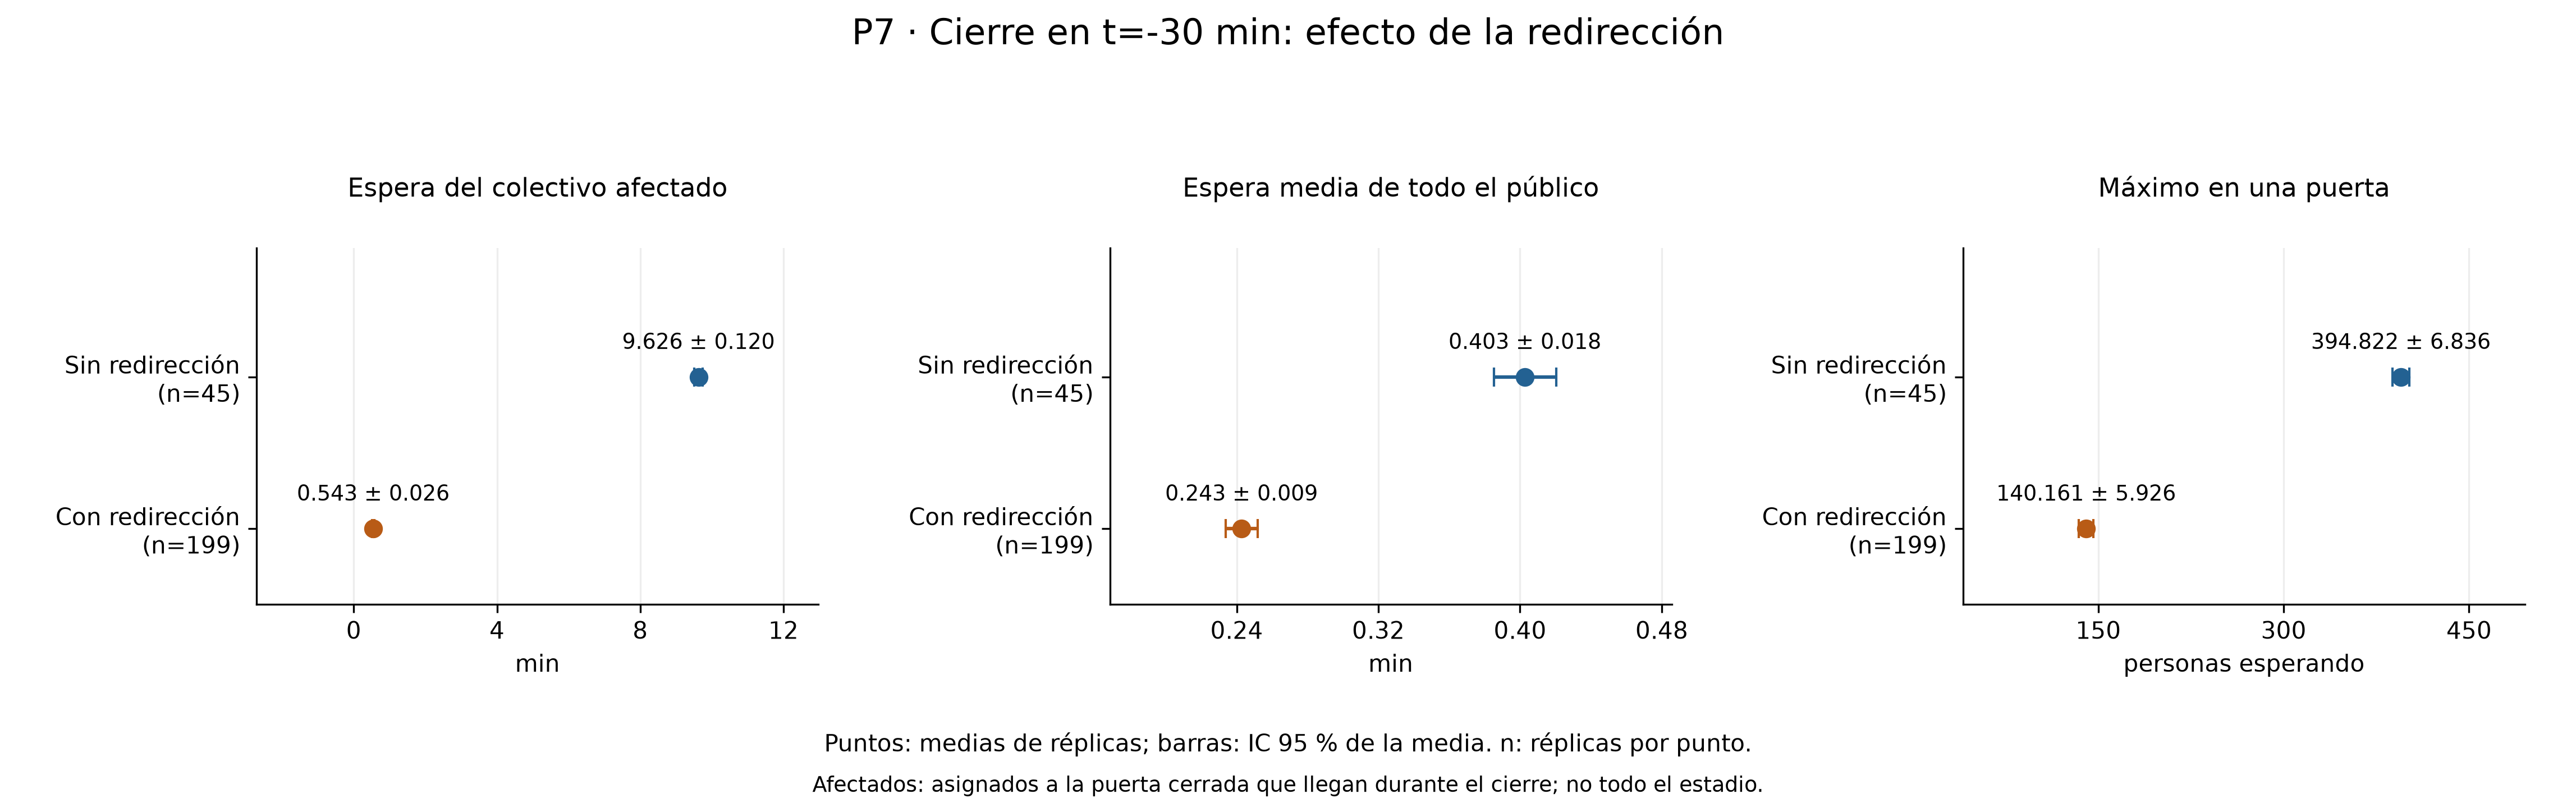
\includegraphics[width=\textwidth]{P7.png}
\caption{P7. Cierre de la puerta A-1 en $[-30,-20)$~min sin redirección ($n=45$) y
con ella ($n=199$): espera del colectivo afectado, espera media de todo el
público y máximo en una puerta. Medias con IC del 95~\%.}
\label{fig:p7}
\end{figure}

Sin redirección, quien llega al cerrar espera casi todo el cierre y quien llega
después se encuentra la cola acumulada; la espera observada coincide con la del
modelo fluido (apartado~\ref{sec:rho}). Con redirección, las otras cinco puertas
de la macrozona reciben un 20~\% más de llegadas durante 10~minutos, con holgura
suficiente ($\rho=0{,}93$), y la espera de los afectados se queda en medio
minuto. La redirección mitiga el cierre, pero no lo hace invisible: frente a X0
sin cierre, la espera media de todo el público con redirección es
$+0{,}050 \pm 0{,}003$~min mayor (180 parejas). El efecto se ve en el colectivo
afectado y en la cola máxima, no en las medias globales, porque el cierre afecta
a 1 de las 24 puertas.

\textbf{Resultado y supuestos.} Que la redirección absorba el cierre es un
resultado del modelo en estas condiciones: hay holgura en las demás puertas en
la punta. La magnitud depende de supuestos que la favorecen.

\textbf{Limitaciones.}
\begin{itemize}
  \item \textbf{Cola ya formada.} Según la hipótesis adoptada
    (sección~\ref{sec:desviaciones}), el cierre solo afecta a quien llega
    mientras dura. En $t=-30$ apenas hay cola formada, así que casi no influye;
    con cierres más tardíos la alternativa daría un efecto mayor, que no se ha
    medido.
  \item \textbf{Redirección optimista.} Quien llega a la puerta cerrada conoce al
    instante la cola de las demás, elige la menor y no camina ninguna distancia
    extra, porque el modelo no representa el exterior. Una redirección real
    costaría tiempo de desplazamiento y no sería perfecta.
  \item \textbf{Un solo caso.} Se ha estudiado una puerta, una duración (10~min) y
    un instante. En $t=+20$, el instante de la Parte 1, el cierre no tenía efecto
    apreciable.
  \item Sin redirección hay 45 réplicas frente a 199 con ella (tamaños por
    precisión); el contraste usa las 45 parejas comunes.
\end{itemize}

% ---------------------------------------------------------------------------
\subsection{P8 · Evacuación de emergencia}

\textbf{Respuesta.} Con todas las salidas el estadio se vacía de media en menos
de 8~minutos, pero no en todos los partidos: falla la marcha de una persona con
movilidad reducida, no la capacidad de las salidas. Con una salida bloqueada no
se cumple en ningún partido.

\begin{table}[htbp]
\centering\small
\caption{Evacuación con alarma en $t=+40$~min (X7, $n=180$ por variante).}
\label{tab:p8}
\begin{tabular}{@{}lrr@{}}
\toprule
Indicador & Todas las salidas & Una salida bloqueada \\
\midrule
Vaciado (min desde la alarma) & 7,469 $\pm$ 0,052 & 8,420 $\pm$ 0,014 \\
Personas a salvo a los 8~min (\%) & 99,9998 $\pm$ 0,0001 & 98,561 $\pm$ 0,028 \\
Partidos vaciados en $\le$ 8~min & 163 de 180 & 0 de 180 \\
\bottomrule
\end{tabular}
\end{table}

\begin{figure}[htbp]
\centering
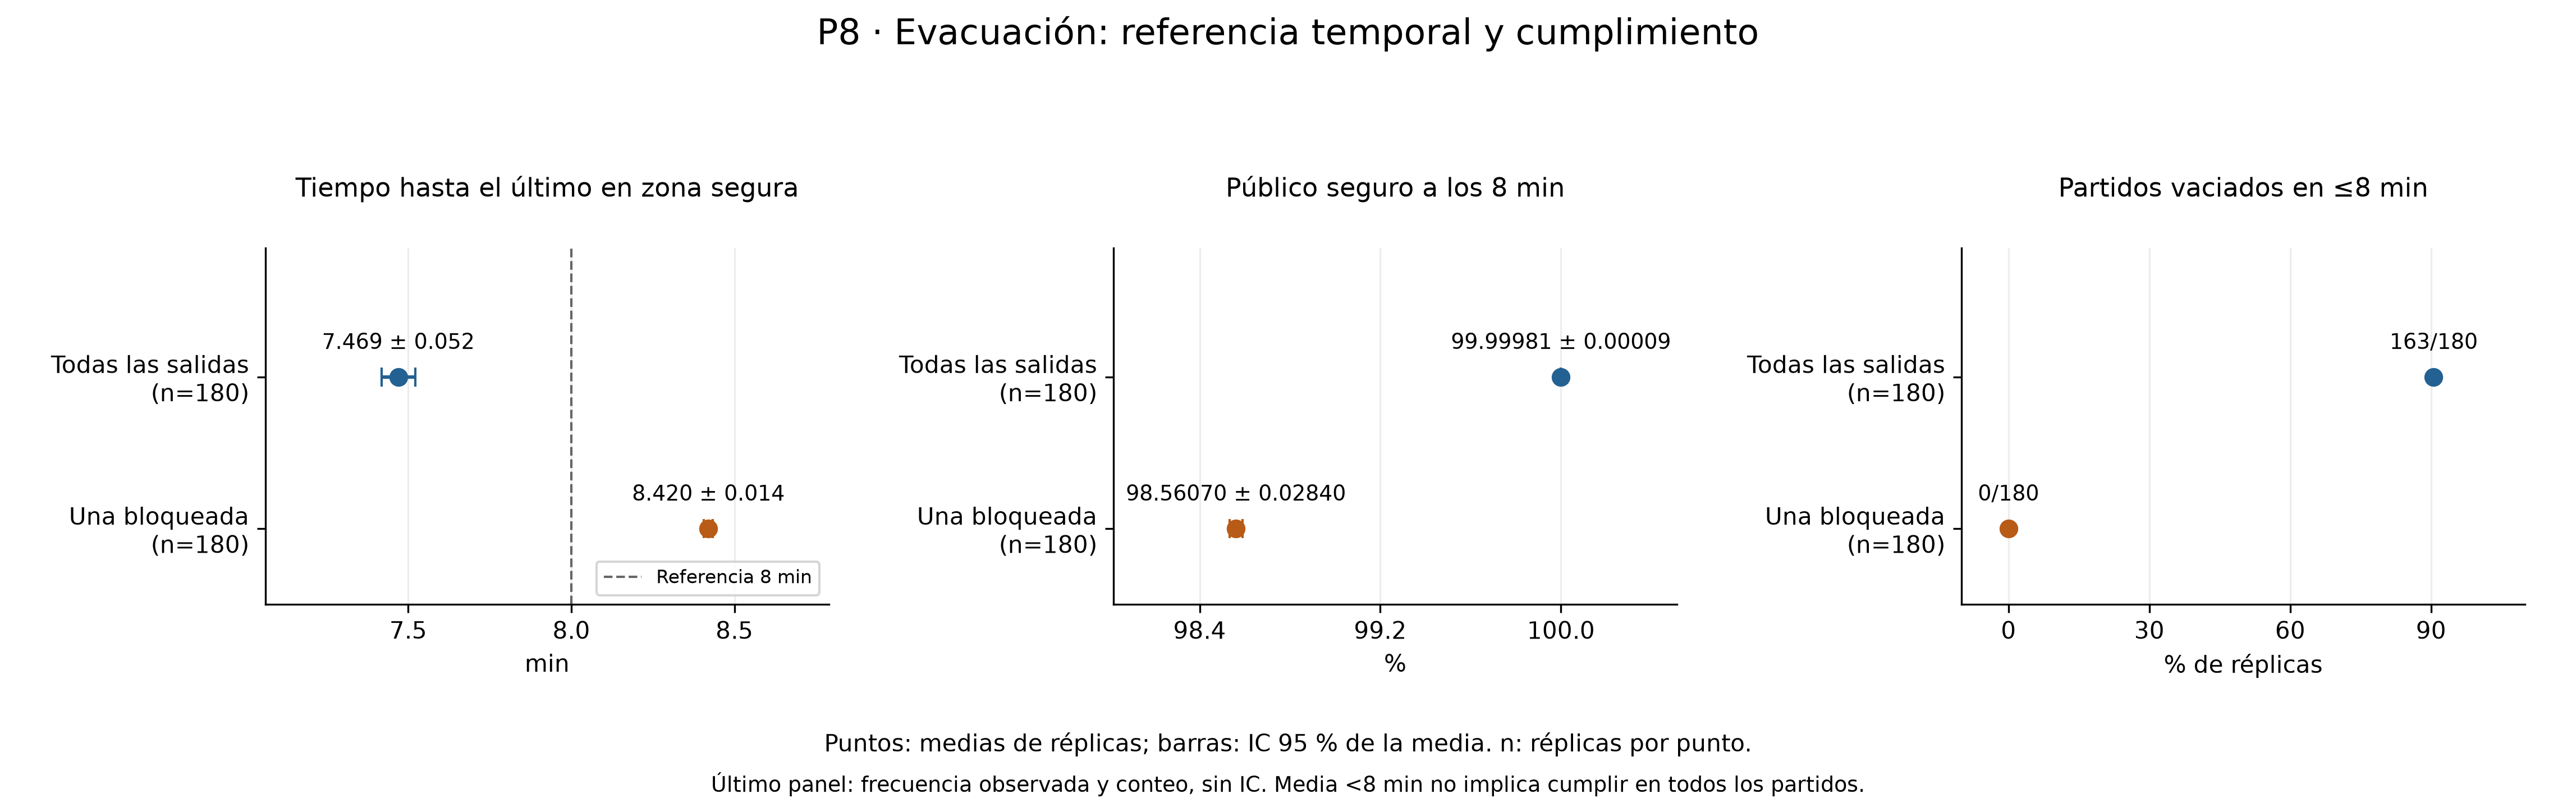
\includegraphics[width=\textwidth]{P8.png}
\caption{P8. Tiempo hasta que el último espectador está a salvo, porcentaje a
salvo a los 8~min y partidos vaciados en ese plazo, con todas las salidas y con
una bloqueada ($n=180$ por variante). Medias con IC del 95~\%; la frecuencia de
partidos se da como recuento, sin IC.}
\label{fig:p8}
\end{figure}

Una media inferior a 8~minutos no garantiza cumplir en cada partido. Con todas
las salidas, en las 17 réplicas que superan el plazo solo llega tarde una
persona, siempre PMR, lejos de la salida y sin hacer cola; sin las PMR, el
vaciado nunca pasa de 7,36~min. La capacidad de las salidas basta y el riesgo
está en evacuar a tiempo a las personas con movilidad reducida. Con una salida
bloqueada sí falla la capacidad: las 5 salidas restantes de la macrozona A no dan
abasto, aunque a los 8~minutos ya está a salvo el 98,56~\% de quienes evacúan.

Estos tiempos son mayores que los 5,9 y 7,1~min de la Parte 1 porque incluyen la
reacción y la marcha hasta la salida, que el cálculo de capacidad excluye.

\textbf{Limitaciones.} No se ha simulado ningún dispositivo de asistencia a las
PMR, así que su eficacia no se puede dar por demostrada. La alarma suena en un
único instante ($t=+40$), con todo el público dentro, y el modelo no representa
densidades, empujones ni bloqueos entre peatones.

\section{Sensibilidad}\label{sec:sensibilidad}

La sensibilidad S1 estudia seis variantes de X0 que cambian un solo factor:
aforo $\pm$10~\%, velocidad de marcha $\pm$15~\% o tiempo de servicio en el torno
$\pm$25~\%. El resto de parámetros es el del escenario base, con salida ordinaria
y sin alarma. Las variaciones no tienen el mismo tamaño entre factores, así que
las diferencias no son una clasificación universal de su importancia, y no se
exploran combinaciones de factores.

\begin{table}[htbp]
\centering\small
\caption{Diferencias emparejadas variante $-$ X0 (min), con IC del 95~\%.}
\label{tab:s1}
\begin{tabular}{@{}lrrrr@{}}
\toprule
Variante & Parejas & Espera media & Tiempo de acceso & Vaciado ordinario \\
\midrule
Aforo $-$10~\% & 180 & $-$0,1036 $\pm$ 0,0050 & $-$0,1085 $\pm$ 0,0051 & $-$0,6734 $\pm$ 0,0342 \\
Aforo $+$10~\% & 73 & $+$0,2867 $\pm$ 0,0114 & $+$0,2924 $\pm$ 0,0112 & $+$0,7604 $\pm$ 0,0228 \\
Velocidad $-$15~\% & 180 & 0 & $+$0,2748 $\pm$ 0,0001 & $+$0,3658 $\pm$ 0,0532 \\
Velocidad $+$15~\% & 180 & 0 & $-$0,1983 $\pm$ 0,0001 & $-$0,0861 $\pm$ 0,0182 \\
Servicio $-$25~\% & 180 & $-$0,1613 $\pm$ 0,0069 & $-$0,1772 $\pm$ 0,0069 & $\approx$ 0 \\
Servicio $+$25~\% & 30 & $+$1,2172 $\pm$ 0,0341 & $+$1,2283 $\pm$ 0,0339 & $\approx$ 0 \\
\bottomrule
\end{tabular}
\end{table}

% La figura S1 tiene tres paneles en una sola imagen; se recortan con trim/clip
% (unidades: bp sobre la imagen de 4590 x 1440 px a 300 ppp) para mostrarlos más
% grandes. No se modifica la imagen ni sus datos.
\begin{figure}[p]
\centering
\begin{subfigure}{\textwidth}\centering
  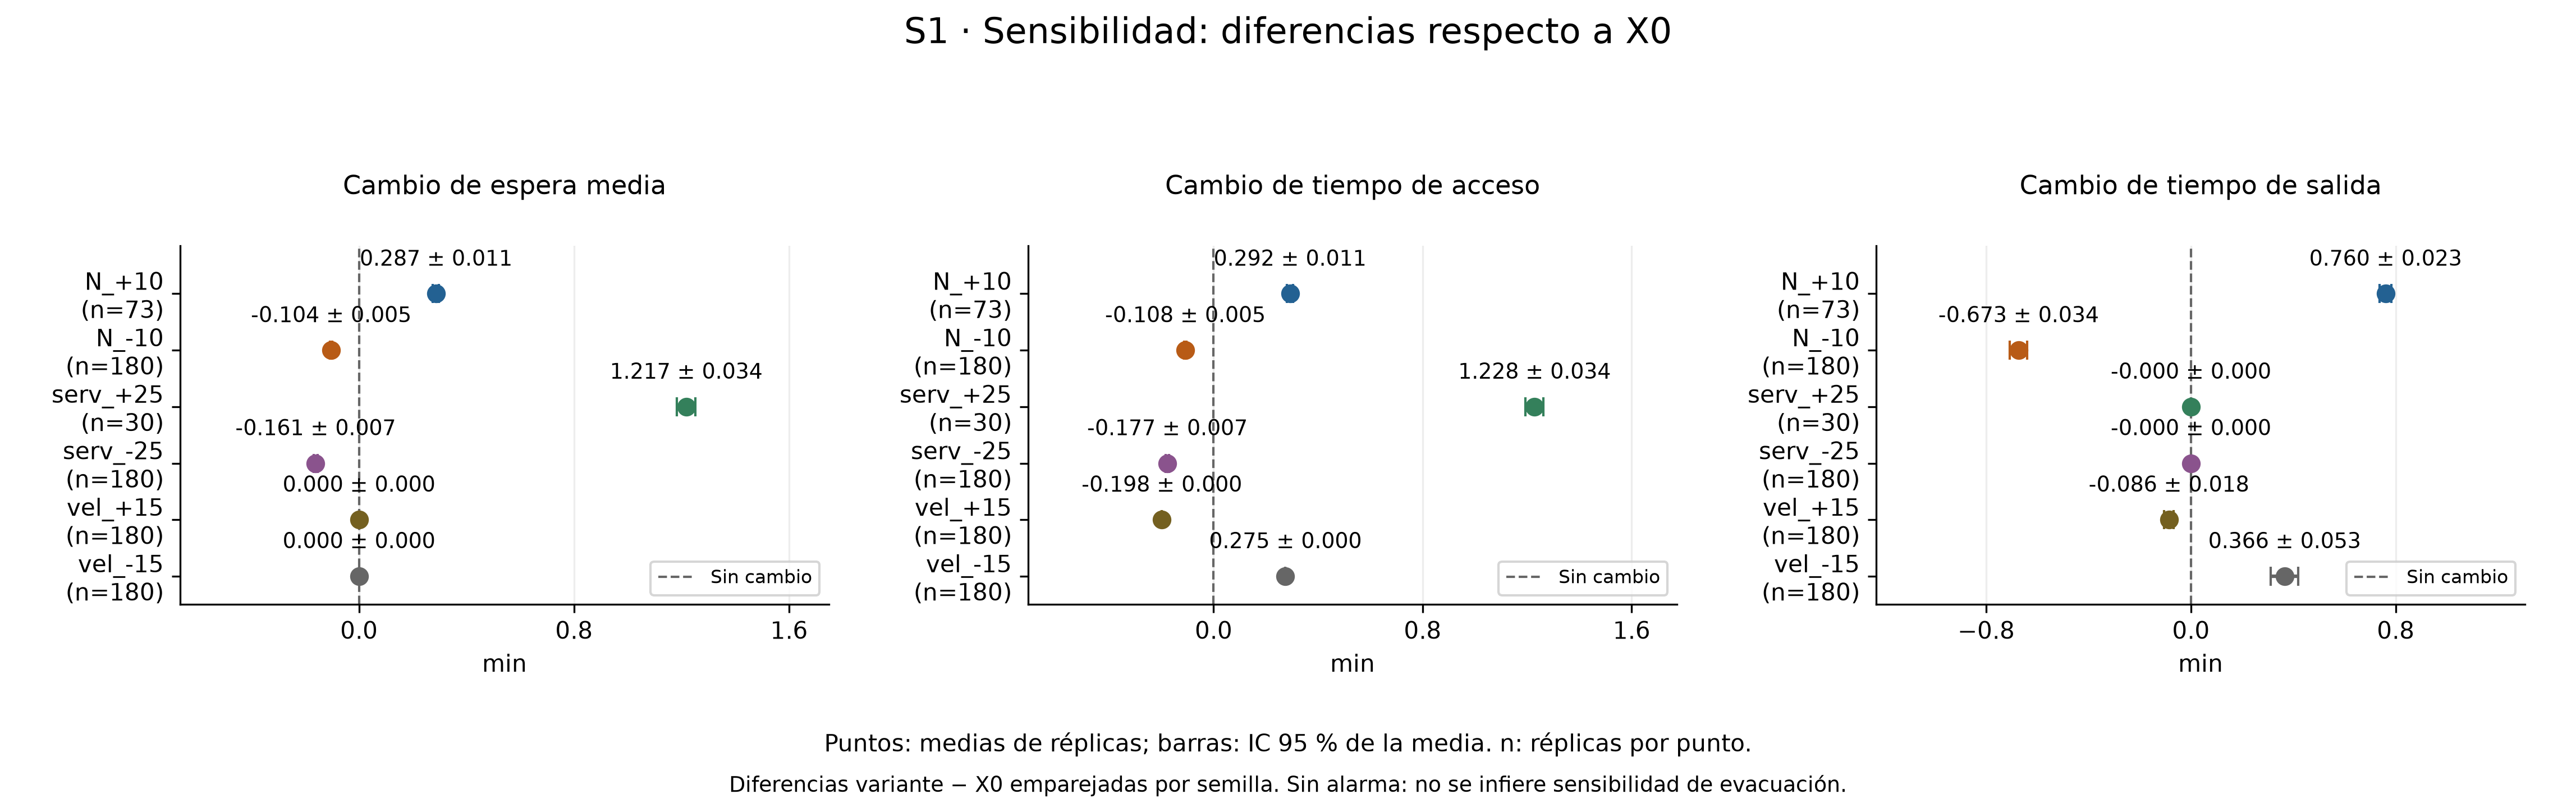
\includegraphics[width=0.66\textwidth,trim=0 57.6 732 72,clip]{S1.png}
  \caption{Cambio de la espera media.}
\end{subfigure}\\[0.6em]
\begin{subfigure}{\textwidth}\centering
  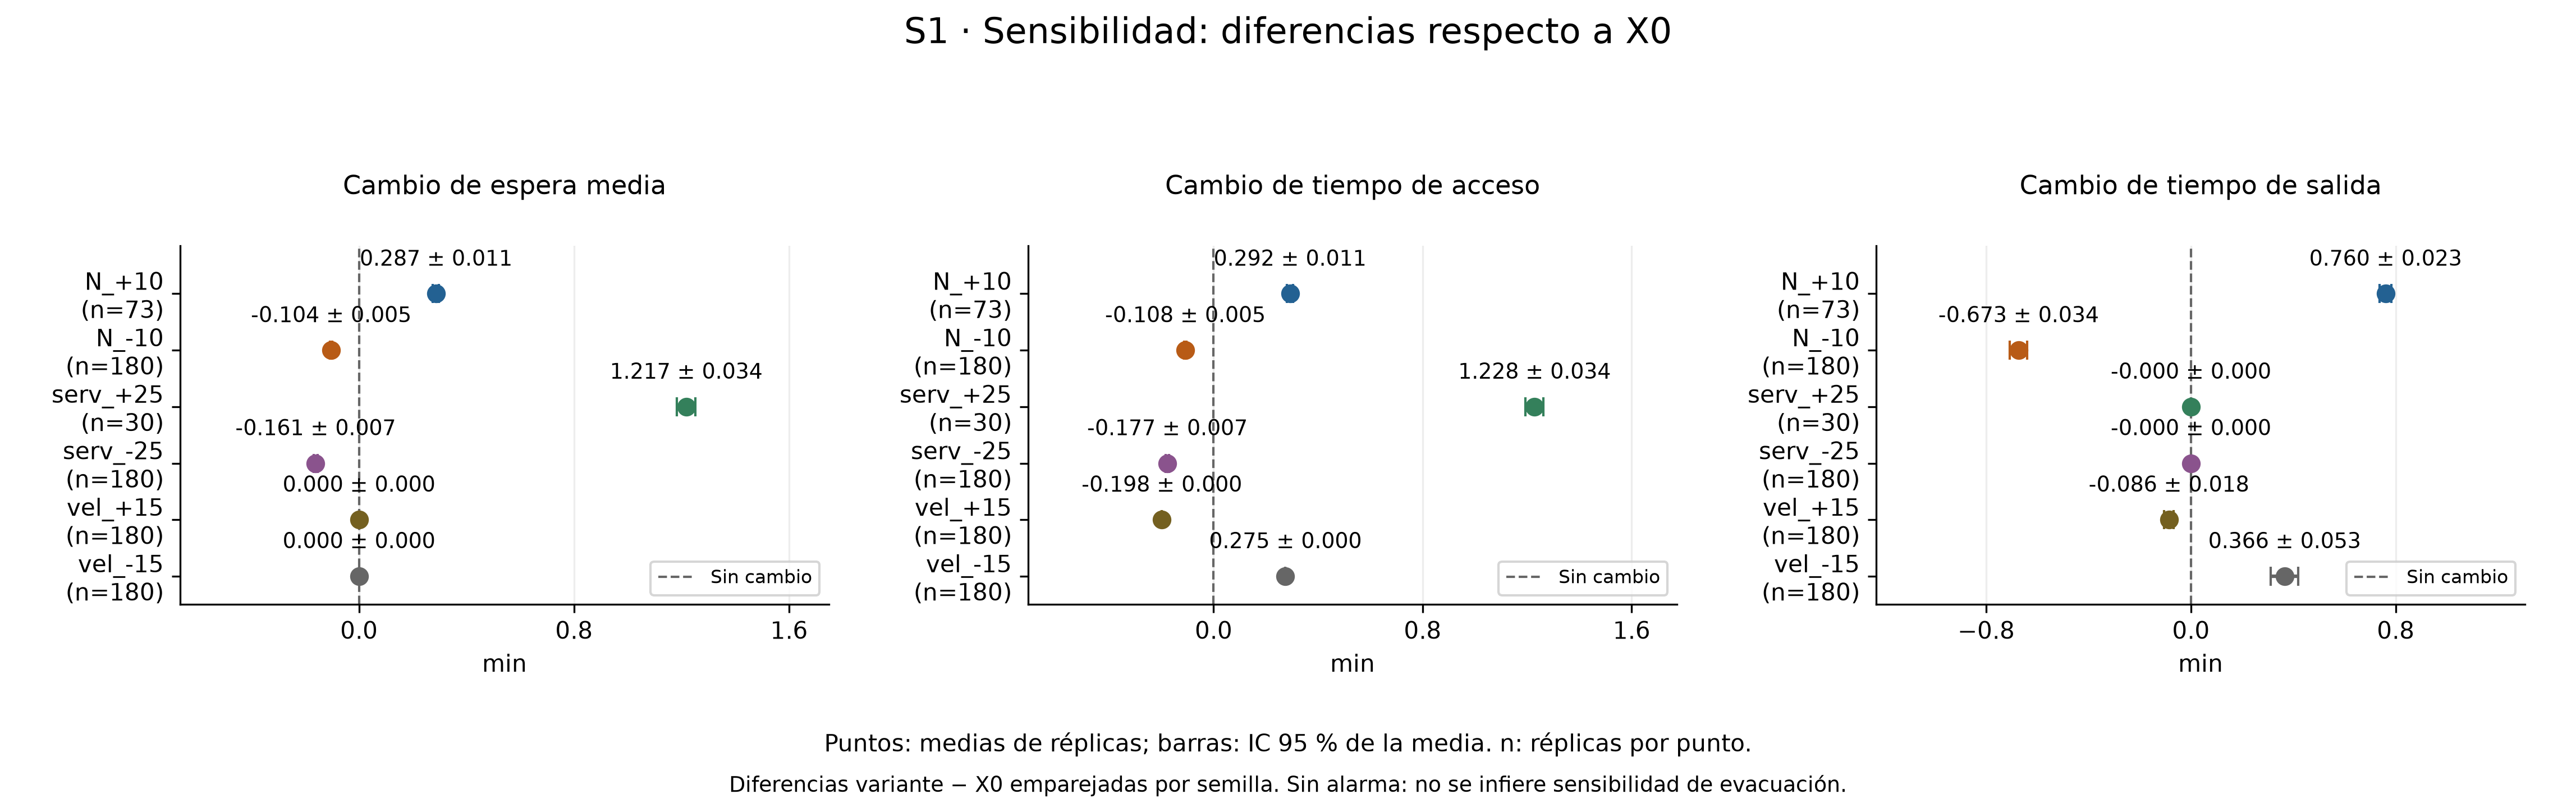
\includegraphics[width=0.66\textwidth,trim=369.6 57.6 369.6 72,clip]{S1.png}
  \caption{Cambio del tiempo de acceso.}
\end{subfigure}\\[0.6em]
\begin{subfigure}{\textwidth}\centering
  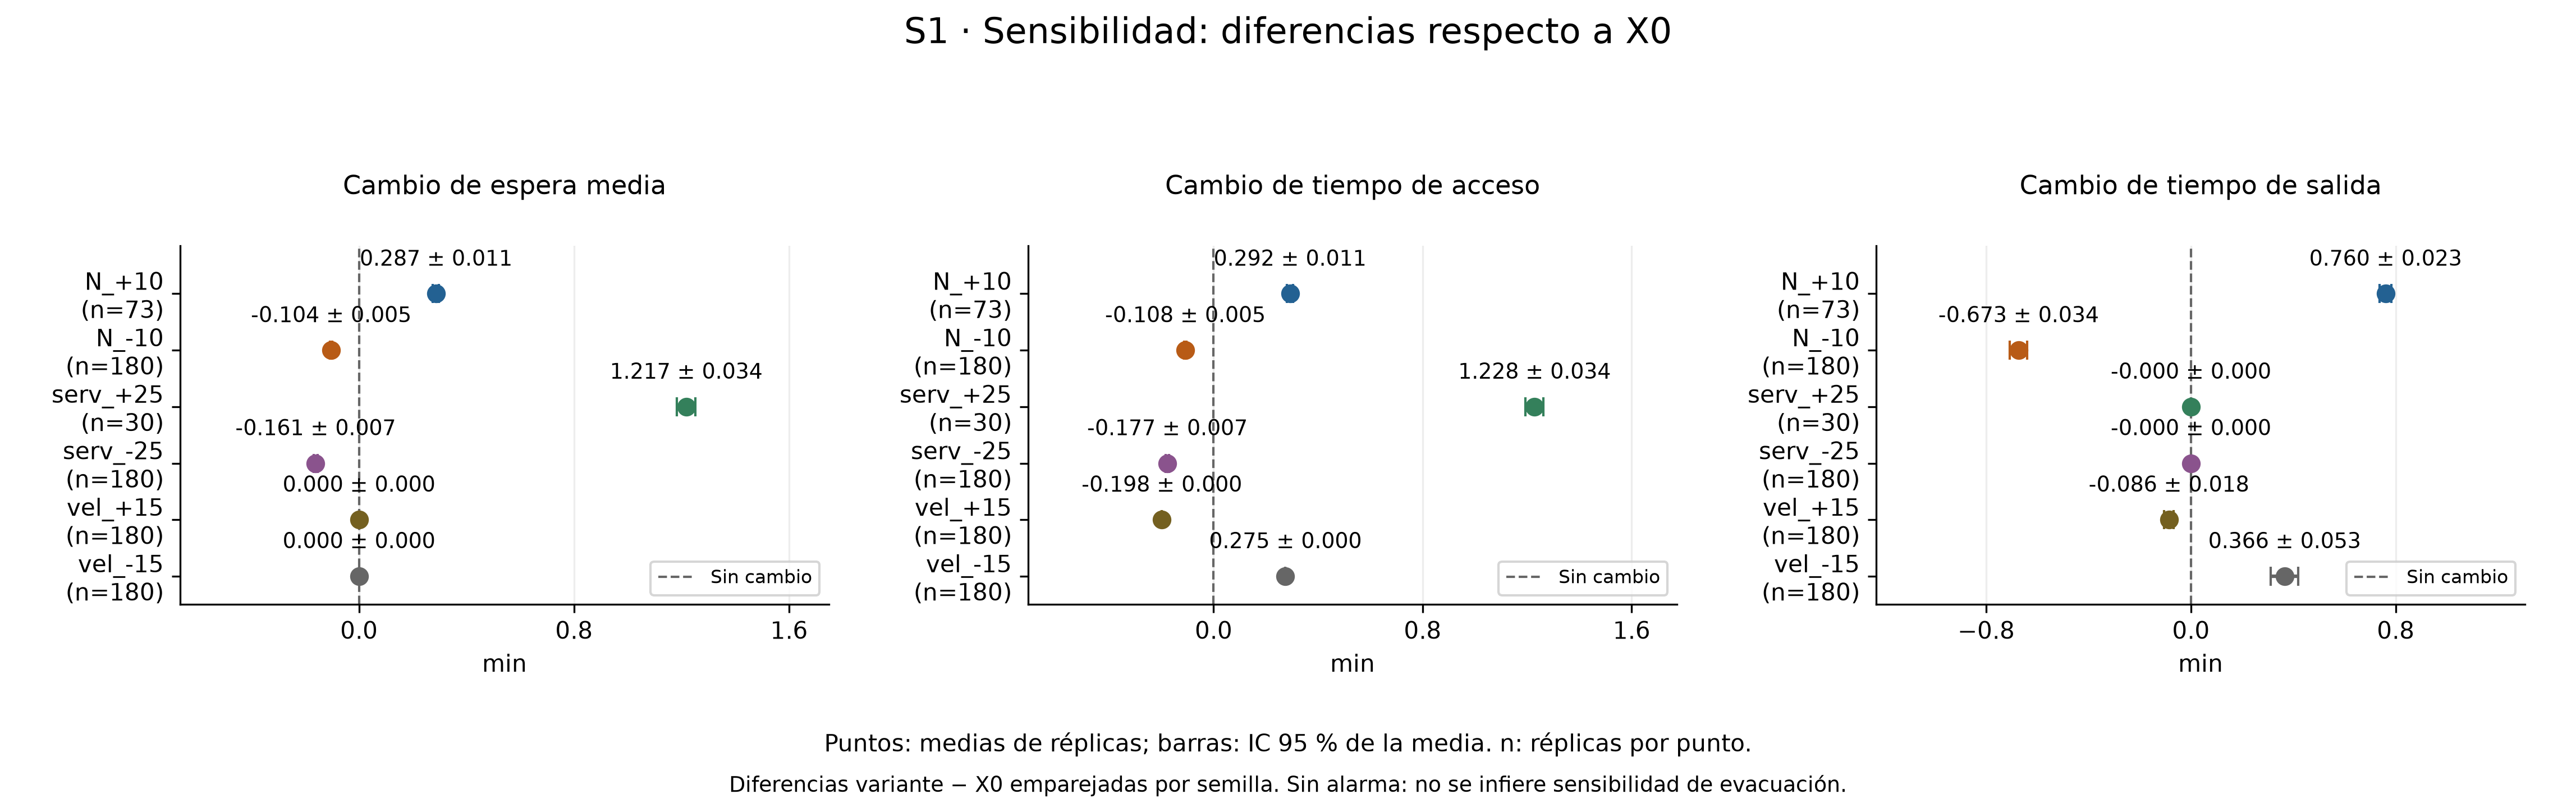
\includegraphics[width=0.66\textwidth,trim=732 57.6 0 72,clip]{S1.png}
  \caption{Cambio del tiempo de vaciado ordinario.}
\end{subfigure}
\caption{S1. Cambio respecto a X0 en cada variante (N: aforo; serv: tiempo de
servicio; vel: velocidad), emparejado por semilla. Puntos: medias; barras: IC
del 95~\%; $n$: parejas por variante (entre 30 y 180). Las variantes no tienen
alarma, así que no indican la sensibilidad de la evacuación.}
\label{fig:s1}
\end{figure}

\textbf{Aforo.} Reducir el público un 10~\% baja la espera media unos 0,104~min;
aumentarlo un 10~\% la sube unos 0,287~min. El efecto no es simétrico porque el
escenario base ya está cerca de la capacidad de entrada en la punta
($\rho=0{,}93$, y 1,02 con un 10~\% más). También cambia el vaciado, porque
cruzan las salidas más o menos personas.

\textbf{Servicio.} Un 25~\% más de tiempo de control sube la espera media unos
1,217~min (unos 73~s) frente a una base de 0,192~min; un 25~\% menos la baja
unos 0,161~min, porque la espera no puede ser negativa. La respuesta a P2 es, por
tanto, sensible al tiempo de servicio supuesto, aunque con 3 tornos el objetivo
se sigue cumpliendo (P2). El vaciado apenas cambia: la entrada termina mucho
antes del final del partido.

\textbf{Velocidad.} No cambia la cola de entrada, que es idéntica semilla a
semilla, porque la marcha ocurre después del control y el modelo no transmite
bloqueos del interior hacia el torno. Sí cambian el acceso y la salida, que
incluyen desplazamientos: la lentitud aumenta el acceso unos 0,275~min y el
aumento de velocidad lo reduce unos 0,198~min, coherente con que el tiempo de
recorrido depende del inverso de la velocidad.

\textbf{Alcance.} S1 permite valorar si algunas conclusiones dependen mucho de
los parámetros inciertos ensayados. No es una calibración con datos reales ni
demuestra robustez frente a cualquier cambio: los IC pequeños solo indican poca
incertidumbre muestral bajo las hipótesis del modelo. Estas variantes no tienen
alarma, así que no son una sensibilidad de la evacuación.

\section{Conclusiones y límites}\label{sec:conclusiones}

\subsection{Conclusiones}

Con los parámetros ensayados, y siempre como comparación entre escenarios:

\begin{itemize}
  \item \textbf{Entrada (P1, P2).} Los tornos son el recurso más cargado, con una
    intensidad de tráfico de 0,93 en la punta. Tres tornos por puerta, el valor
    actual, cumplen el objetivo de espera y dos no; el margen es sensible al
    tiempo de servicio.
  \item \textbf{Llegada anticipada (P3).} Reduce la espera y, sobre todo, la
    entrada tardía, que depende más de cuándo llega el público y del recorrido
    hasta el asiento que de la cola del torno.
  \item \textbf{Prioridad (P4).} Beneficia a mayores y PMR con un coste pequeño y
    repartido para el resto, sin cambiar la espera total.
  \item \textbf{Salida escalonada (P5).} Reduce casi a la mitad la aglomeración en
    las salidas a cambio de alargar algo más de un minuto el vaciado.
  \item \textbf{Acomodadores (P6).} Son decisivos cuando se duplica la probabilidad
    de conflicto: con 3 por macrozona el sistema se satura y con 9 la duración de
    un conflicto se acerca a la de su resolución.
  \item \textbf{Cierre de puerta (P7).} La redirección a la puerta con menos cola
    absorbe casi todo el efecto de un cierre en la punta, en condiciones
    favorables a la redirección.
  \item \textbf{Evacuación (P8).} Con todas las salidas la capacidad basta, pero no
    siempre se evacúa a tiempo a las personas con movilidad reducida; con una
    salida bloqueada no se cumple la referencia de 8~minutos. El promedio de
    vaciado, por sí solo, no responde a la pregunta.
\end{itemize}

Estas conclusiones deben acompañarse de los IC, los tamaños por escenario y los
límites siguientes.

\subsection{Límites}

\begin{itemize}
  \item \textbf{Validación externa.} La verificación comprueba conservación,
    orden, capacidades, casos límite, cálculo de indicadores y reproducibilidad.
    No hay datos completos de colas, salida y evacuación con los que cuantificar
    el error respecto al estadio real. El ritmo por torno se ha contrastado con la
    cifra que la Parte 1 atribuye a la fuente F2, sin volver a comprobarla en el
    artículo original.
  \item \textbf{Precisión.} El criterio de precisión controla la incertidumbre
    muestral de la espera media; no controla el error de los parámetros, de la
    representación espacial ni de las reglas de comportamiento.
  \item \textbf{Generalización.} Las decisiones se estudian con perfiles,
    probabilidades y recursos concretos: no cabe generalizar que tres tornos
    basten para cualquier demanda ni que nueve acomodadores sean siempre
    suficientes.
  \item \textbf{Representación espacial.} El exterior del estadio no está
    representado y la redirección no añade marcha ni información imperfecta.
    Los peatones tienen velocidades y distancias sorteadas, sin un modelo de
    densidad, empujones o asistencia. Esto afecta sobre todo a P7 y P8.
  \item \textbf{Hipótesis adoptadas.} En particular, que el cierre de una puerta
    solo afecta a quien llega mientras dura (sección~\ref{sec:desviaciones}).
    No influye con el cierre estudiado, pero no se ha comprobado con cierres
    posteriores ni con una redirección menos favorable.
  \item \textbf{Sensibilidad.} S1 cambia cada factor por separado y no incluye la
    emergencia; no responde a combinaciones de aforo, servicio y velocidad ni a
    medidas de evacuación asistida.
\end{itemize}

\section*{Referencias}
\addcontentsline{toc}{section}{Referencias}

\begin{description}[style=nextline,leftmargin=2.2em,font=\bfseries\color{azul}]
  \item[F1] Athletic Club. «San Mamés». Web oficial del estadio.
    \url{https://sanmames.athletic-club.eus/san-mames/}
  \item[F2] García, A.; Guerrero, B.\,V.; Hernández-Delfin, D.; Lee, D.\,J.; Ellero, M. (2026).
    «Modeling crowd flow during stadium ingress under alternative access protocols:
    San Mamés as a case study». \emph{Simulation Modelling Practice and Theory}, 149,
    103279. \url{https://doi.org/10.1016/j.simpat.2026.103279}
  \item[F3] Athletic Club (15/09/2025). «Indicaciones para el acceso a San Mamés en el
    Athletic Club -- Arsenal FC».
    \url{https://www.athletic-club.eus/noticias/2025/09/15/indicaciones-para-el-acceso-a-san-mames-en-el-athletic-club-arsenal-fc/}
  \item[F4] SimPy. Documentación oficial de SimPy (recursos compartidos, procesos e
    interrupciones). \url{https://simpy.readthedocs.io/}
  \item[F5] Sports Grounds Safety Authority. «Egress». \emph{Guide to Safety at Sports
    Grounds -- Green Guide}, cap.~10. \url{https://sgsa.org.uk/physical-factors/circulation/egress/}
  \item[F6] Northern Ireland Assembly, Research and Information Service (2015). «An
    outline of stadium safety legislation and guidance».
    \url{https://www.niassembly.gov.uk/globalassets/documents/cal/inquiry/casement-park/research-papers/an-outline-of-stadium-safety-legislation-and-guidance-9.6.15.pdf}
  \item[D1] Diseño de Modelos de Simulación. Guion de Prácticas, curso 2026/2027.
\end{description}


\end{document}
